%%
%% This is file `03_article2.tex',
%% generated with the docstrip utility.
%%
%% The original source files were:
%%
%% dms.dtx  (with options: `article')
 
%% To change chapter header dynamically from french to english, use
\entetedynamique
\setcounter{corA}{0} % Pour recommancer à compter les def,
                     % theo, etc. à partir de 1

\setcounter{figure}{0}
\renewcommand{\thefigure}{\arabic{chapter}.\arabic{figure}}

 % Pour écrire un article en français
\francais
 % Pour écrire un article en anglais
%% \anglais
%% NOTE: La plupart des macros ont un nom en anglais.
%% P.ex. \adresse et \address fonctionnent et sont équivalents.
%% \revue=\journal
%% \auteur=\author
%% \titre=\title

%% Les contributions apparaîtront habituellement après
%% \maketitle (voir un peu plus bas). Selon les goûts, il est
%% possible de mettre les contributions
%% avant la page titre de l'article, simplement en les écrivant
%% directement ici. Par exemple :
 % \cleardoublepage
 % \pdfbookmark[chapter]{Contributions}{contrib1} % Remplacer par contrib2 pour l'article 2 etc.
 % {\bfseries\Large\noindent Contributions de <mon nom> et rôle joué par les coauteurs}
 % J'ai contribué en...
 %
 % Le rôle des coauteurs a été de...

%% Nom de la revue de publication
\revue{PLOS Computational Biology et est accessible via le lien suivant : \url{https://doi.org/10.1371/journal.pcbi.1011458}}
\article{What constrains food webs? A maximum entropy framework for predicting their structure with minimal biases}\labelart{art:article2}
%% On peut se référer aux numéros de chapitre ou d'article comme suit.
%% Si on fait
%% \label{chap:article1},
%% alors \ref{chap:article1} donnera le numéro du chapitre. On peut ensuite faire
%% \labelart{art:article1}
%% et alors \ref{art:article1} donnera le numéro d'article.
%% Par exemple, si cette article est le premier article et le deuxième chapitre,
%% alors si on écrit
%% Voir le chapitre~\ref{chap:article1} (l'article~\ref{art:article1}).
%% deviendra
%% Voir le chapitre 2 (l'article 1).
%% Si on veut écrire « premier article » au lieu « article 1 », on peut
%% simplement faire
%% \ordinal{\ref{art:article1}}~article  % devient première article
%% ou
%% \Ordinal{\ref{art:article1}}~article  % devient Première article (avec la majuscule)
%% Si on est en mode \anglais, \ordinal écrire first, second,...

 % Contribution(s) personnelle(s) à l'article et rôle joué par tous les coauteur·e·s
 %
 % Nécessaire seulement lorsque vous n'êtes pas seul·e auteur·e.
 % Les contributions peuvent apparaître ailleur dans la thèse.
 % Si \contributions est laissé vide (p.ex. si vous effacez
 % celui ci-bas), aucune contributions ne seront générées sur
 % la page titre de l'article. Vous pouvez alors mettre un
 % \newpage si vous souhaitez que les résumé et abstract soient
 % la page suivante.
 %
 % REMARQUE : À peu près toutes les constructions \LaTeX\ sont permises
 % dans les contributions.
 %
 % La commande admet une option [<entête>]
\contributions%[Mes contributions et le rôle des coauteurs]
{
  Francis Banville a développé et réalisé les analyses et a rédigé les versions
  initiale et finale du manuscrit. Dominique Gravel et Timothée Poisot ont
  fourni des conseils sur les analyses et l'interprétation des résultats et ont
  révisé le manuscrit. Tous les auteurs ont lu et approuvé le manuscrit.\\[1cm]
  
  %  \begin{itemize}
  %      \item Calcul de telle chose;
  %      \item Vérification de telle équation;
  %      \item Idée pour telle définition;
  %      \item Démonstration de tel théorème.
  %  \end{itemize}
}

%%% INFORMATIONS POUR LA PAGE TITRE
 % Premier auteur·e et adresse
\auteur{Francis Banville}
\adresse{Département de sciences biologiques, Université de Montréal
\\1375 avenue Thérèse-Lavoie-Roux, Montréal, QC, Canada H2V 0B3}
 
 % Deuxième auteur·e et adresse (si différente de la première)
\auteur{Dominique Gravel}
\adresse{Département de biologie, Université de Sherbrooke
\\2500 boulevard de l'Université, Sherbrooke, Qc, Canada J1K 2R1}
%%
%% et ainsi de suite pour les autres auteurs

\auteur{Timothée Poisot}
\adresse{Département de sciences biologiques, Université de Montréal
\\1375 avenue Thérèse-Lavoie-Roux, Montréal, QC, Canada H2V 0B3}

\maketitle

\begin{resume}{modélisation écologique, réseaux écologiques, réseaux trophiques, entropie maximale, modèles nuls}
  Les réseaux trophiques sont des réseaux complexes dont la structure est
  écologiquement et statistiquement contrainte, plusieurs de leurs propriétés
  émergentes étant fortement corrélées entre elles. Malgré la reconnaissance de
  ces relations invariantes au sein des réseaux trophiques, l'utilisation du
  principe d'entropie maximale (MaxEnt) en écologie des réseaux est rare. Cela
  est surprenant étant donné que MaxEnt est un outil statistique conçu
  spéficiquement pour comprendre et prédire de nombreux types de systèmes
  contraints. Ce principe stipule que la distribution de probabilité la moins
  biaisée d'une propriété d'un système, contrainte par nos connaissances
  préalables sur ce système, est celle avec l'entropie d'information maximale.
  MaxEnt s'est révélé utile dans de nombreux problèmes de modélisation
  écologique, mais son application aux réseaux trophiques et écologiques est
  limitée. Ici, nous montrons comment MaxEnt peut être utilisé pour dériver de
  nombreuses propriétés des réseaux trophiques, à la fois analytiquement et
  heuristiquement. Premièrement, nous montrons comment la distribution conjointe
  des degrés (la distribution de probabilité conjointe des nombres de proies et
  de prédateurs pour chaque espèce dans le réseau) peut être dérivée
  analytiquement en utilisant le nombre total d'espèces et d'interactions des
  réseaux trophiques. Deuxièmement, nous présentons une approche heuristique et
  flexible pour trouver la matrice d'adjacence d'un réseau (la représentation du
  réseau sous forme de matrice) en utilisant la méthode de recuit simulé et
  l'entropie SVD. Nous avons construit deux modèles heuristiques utilisant
  respectivement la connectance et la séquence de degrés conjointe comme
  contraintes statistiques. Nous avons comparé les prédictions des deux modèles
  à celles de modèles nuls et neutres couramment utilisés en écologie des
  réseaux en utilisant des données en accès libre de réseaux trophiques
  terrestres et aquatiques échantillonnés à l'échelle globale (N = 257). Nous
  avons constaté que le modèle heuristique contraint par la séquence de degrés
  conjointe était un bon prédicteur de nombreuses mesures de la structure des
  réseaux trophiques, en particulier l'emboîtement et la distribution des
  motifs. Plus précisément, nos résultats suggèrent que la structure des réseaux
  trophiques terrestres et aquatiques est principalement déterminée par leur
  distribution conjointe de degrés.
\end{resume}

\begin{abstract}{ecological modelling, ecological networks, food webs, maximum entropy, null models}
  Food webs are complex ecological networks whose structure is both ecologically
  and statistically constrained, with many network properties being correlated
  with each other. Despite the recognition of these invariable relationships in
  food webs, the use of the principle of maximum entropy (MaxEnt) in network
  ecology is still rare. This is surprising considering that MaxEnt is a
  statistical tool precisely designed for understanding and predicting many
  types of constrained systems. This principle asserts that the least-biased
  probability distribution of a system's property, constrained by prior
  knowledge about that system, is the one with maximum information entropy.
  MaxEnt has been proven useful in many ecological modeling problems, but its
  application in food webs and other ecological networks is limited. Here we
  show how MaxEnt can be used to derive many food-web properties both
  analytically and heuristically. First, we show how the joint degree
  distribution (the joint probability distribution of the numbers of prey and
  predators for each species in the network) can be derived analytically using
  the number of species and the number of interactions in food webs. Second, we
  present a heuristic and flexible approach of finding a network's adjacency
  matrix (the network's representation in matrix format) based on simulated
  annealing and SVD entropy. We built two heuristic models using the connectance
  and the joint degree sequence as statistical constraints, respectively. We
  compared both models' predictions against corresponding null and neutral
  models commonly used in network ecology using open access data of terrestrial
  and aquatic food webs sampled globally (N = 257). We found that the heuristic
  model constrained by the joint degree sequence was a good predictor of many
  measures of food-web structure, especially the nestedness and motifs
  distribution. Specifically, our results suggest that the structure of
  terrestrial and aquatic food webs is mainly driven by their joint degree
  distribution.
\end{abstract}

\clearpage 

\section{Introduction}
%%
%%
% Exemple de citation~: Consultez le \LaTeX\ companien
% de Mittelbach {\it et al\/}~\cite{exemple}.

%Imports bibliography file

\subsection{The constrained structure of ecological networks}

A variety of measures of the structure of ecological networks have been used to
describe the organization of species interactions in a biological community
(\cite{Delmas2019Analysing}). These measures provide valuable information on the
functioning of ecosystems and their responses to environmental change (e.g.
\cite{Pascual2006Ecological}, \cite{Gomez2011Functional}). For instance, two main
properties of a network are its order (the number of nodes or species $S$) and
its size (the number of edges or species interactions $L$), whose ratio $L/S^2$
(the proportion of possible interactions that are realized) is called
connectance. In food webs, \textcite{Dunne2002Network} showed that a high
connectance can promote the robustness of the community to species lost.
Moreover, a different investigation of network structure revealed that
plant–pollinator and seed-disperser networks have a highly nested structure that
can promote species persistence (\cite{Bascompte2003Nested}). Despite the
recognition of the ecological significance of network structure, our knowledge
of the properties of ecological networks remains limited and is unevenly
distributed across space (\cite{Poisot2021Global}). This can largely be
attributed to the difficulties encountered when sampling interactions
(\cite{Jordano2016Sampling}), which impede our ability to describe network
structure on a global scale. Moreover, these complex systems
(\cite{Williams2000Simple}) have an emerging structure with intricate dynamics
(i.e. non-linear behaviors that cannot be predicted from individual
interactions). Their multi-faceted nature and high level of complexity represent
a challenge when studying the ecological processes driving their structure,
especially given the strong relationship between many of their properties. For
example, nestedness and modularity are highly correlated in ecological networks
(\cite{Fortuna2010Nestedness}) and many emerging properties are linked to
connectance (\cite{Poisot2014When}). In light of these observations, it is
difficult to assess whether the presumed effects of a particular measure on
network structure and behavior are the artifacts of other, perhaps simpler,
measures.

One way to address this issue is to recognize that food webs and other
ecological networks are constrained systems. In other words, the space of
possible network configurations is shaped by our partial knowledge of their
structure. For example, there is a finite set of networks with a given number of
species and interactions (i.e. a given connectance). As shown by
\textcite{Poisot2014When}, connectance can constrain many aspects of network
structure such as the degree distribution (i.e. the probability distribution of
the number of interactions realized by a species). Because of the scaling
relationship between the total number of species and interactions, network
structure is also largely constrained by its order (food webs with high species
richness typically have a low connectance compared to smaller networks,
\cite{MacDonald2020Revisiting}). Other measures, such as the maximum trophic level
(i.e. the maximum number of times energy is transformed along food chains
through biomass consumption), may also constrain the space of feasible networks,
e.g. by imposing a limit on energy transfer (\cite{Williams2004Limits}). 

Prior knowledge of the structure of ecological networks, even partial, can be
useful in the current context of data scarcity about species interactions. The
Eltonian shortfall, which describes the gap between our present-day knowledge of
ecological networks and a comprehensive understanding of interactions
(\cite{Hortal2015Seven}), can be partially alleviated using known information
about a network's attributes. First, knowing a given set of network properties
(e.g. the number of species and interactions), it is possible to identify
various structures that meet these constraints and estimate their respective
probabilities of occurrence. For instance, a set of adjacency matrices (i.e. a
representation of interactions in matrix format) that satisfy the known
properties can be found. Selecting the right adjacency matrix among all of these
suitable configurations or evaluating their relative probabilities may be done
using different modeling tools (e.g. using the principle of maximum entropy or
Bayesian inference). Second, as suggested by \textcite{Strydom2021Roadmapa}, network
structure can also be used to facilitate the estimation of pairwise species
interactions. For example, by knowing a network's adjacency matrix (or the
constrained space of feasible networks), we can decrease the volume of
information we need to infer interactions (e.g. by knowing how many prey each
species should have). Moreover, network structure can be used as validation to
ensure that inferred interactions collectively satisfy known structural
properties. Overall, partial knowledge of a network's properties can help us
reconstruct its emerging structure and individual interactions when data is
lacking. 

Predicting ecological networks and understanding the biological mechanisms that
shape species interactions are two complementary aims of network ecology. On one
hand, prediction is the process of estimating the value of an unknown variable
using available data and appropriate statistical models and assumptions. The
goal of predictive models is to minimize predictive errors and provide reliable
estimates of the unknown variable. These models have the potential to fill many
data gaps about species interactions and network structure by making sound
predictions and generating new data. A variety of such models have recently been
developed using machine learning and other statistical tools, most of which are
presented in \textcite{Strydom2021Roadmapa}. On the other hand, statistical models can
also be built to describe or understand a parameter or mechanism of interest.
For example, null models are statistical models that generate baseline
distributions to evaluate the significance of an observed measure. These
distributions are obtained from different randomizations of a network that
maintain some of its properties while deliberately omitting others. By assessing
the deviation of empirical data from these reference distributions, we can
evaluate the degree to which the processes underlying the null model can
accurately capture the observed measures, providing a benchmark to assess the
importance of additional factors such as the omitted properties
(\cite{Fortuna2006Habitat}, \cite{Delmas2019Analysing}). This makes null models a
valuable tool to identify the ecological mechanisms that drive species
interactions and constrain the structure of ecological networks. The distinction
between understanding and predicting is crucial when using statistical and
mathematical models as this can impact how we use and interpret them. Numerous
predictive and null models have been used to analyze ecological networks
(\cite{Delmas2019Analysing}, \cite{Strydom2021Roadmapa}). Nevertheless, given the
constrained nature of ecological networks, it is surprising that the principle
of maximum entropy, a mathematical method designed for both the description and
prediction of constrained systems, has been barely used in network ecology. 

\subsection{The principle of maximum entropy: A primer for ecologists}

The principle of maximum entropy (MaxEnt) is a mathematical method of finding
probability distributions, strongly rooted in statistical mechanics and
information theory (\cite{Jaynes1957Information}, \cite{Jaynes1957Informationa},
\cite{Harremoes2001Maximum}). Starting from a set of constraints given by prior
knowledge of a system (i.e. what we call state variables), this method helps us
find least-biased probability distributions subject to the constraints. These
probability distributions are guaranteed to be unique given our prior knowledge
and represent the most we can say about a system without making more
assumptions. For example, if we know the number of species and total number of
individuals in a biological community (our state variables), we can calculate
the average number of individuals per species (our constraint). Using the
principle of maximum entropy, one could show that the least-biased species
abundance distribution (i.e. the distribution of the number of individuals of
each species), constrained by the average species abundance, follows an
exponential distribution whose parameter is determined by the values of the
state variables (\cite{Frank2011Simple}, \cite{Harte2014Maximum}). However,
this does not imply that this distribution will be the best fit to empirical
data. The challenge is to find the right set of constraints that would best
reproduce distributions found in nature. 

MaxEnt states that the least-biased probability distribution given the
constraints used is the one with the highest entropy (a measure of the
uncertainty of a random process) among all probability distributions that
satisfy these constraints. Many measures of entropy have been developed in
physics (\cite{Beck2009Generalised}), but only a fraction of them could be used as
an optimization measure with the principle of maximum entropy. According to
\textcite{Beck2009Generalised} and \textcite{Khinchin2013Mathematical}, a measure of entropy $H$
should satisfy four properties: (1) it should be a function of a probability
distribution $p(n)$ only; (2) it should be maximized when $p(n)$ is uniform; (3)
it should not be influenced by outcomes with a null probability; and (4) it
should be independent of the order of information acquisition. The Shannon's
entropy (\cite{Shannon1948Mathematical})

\begin{eqnarray}
  \label{eq:shannon}
          H = -\sum_{n} p(n) \log p(n)
\end{eqnarray}

satisfies all of these properties. Finding the probability distribution $p(n)$
that maximizes $H$ under a set of $m$ constraints $g$ can be done using the
method of Lagrange multipliers. These constraints can include one or many
properties of the probability distribution (e.g. its mean, variance, and range).
However, the normalization constraint always needs to be included in $g$ to make
sure that $p(n)$ sums to $1$. The objective is then to find the values of the
Lagrange multipliers $\lambda_i$ that optimize a function $F$: 

\begin{eqnarray}
  \label{eq:F}
          F = H - \sum_{i=1}^m \lambda_i (g_i-c_i),
\end{eqnarray}
  
where $g_i$ is the mathematical formulation of the constraint $i$ and $c_i$,
its value. Note that $F$ is just Shannon's entropy to which we added terms
that each sums to zero ($g_i = c_i$). $F$ is maximized by setting to $0$ its
partial derivative with respect to $p(n)$. 

The principle of maximum entropy has been used in a wide range of disciplines,
from thermodynamics, chemistry and biology (\cite{Martyushev2006Maximum}) to
graph and network theory (e.g., \cite{Park2004Statistical},
\cite{vanderHoorn2018Sparse}). MaxEnt has also been proven useful in ecology,
e.g. in species distribution (\cite{Phillips2006Maximum}) and macroecological
(\cite{Harte2008Maximum}, \cite{Harte2014Maximum}) models. In network ecology,
it can be used to generate null models of network structure with either fixed or
fluctuating constraints (\cite{Caruso2022Fluctuating}) and predict important
network properties using limited data. For example, it has been used to predict
the degree distribution of bipartite networks from the number of species and the
number of interactions (\cite{Williams2011Biology}) and the strength of biotic
interactions from species relative abundances (\cite{Stock2021Optimal}).
However, to the best of our knowledge, MaxEnt has never been used to predict
food-web structure directly, even though food webs are among the most documented
and widespread ecological networks (\cite{Ings2009Review}).

Food-web properties that can be derived using MaxEnt are varied and pertain to
different elements of the network (i.e. at the species, interaction and
community levels). Because MaxEnt is a method of finding least-biased
probability distributions given partial knowledge about a system, these
properties need to be represented probabilistically. For example, at the species
level, MaxEnt can be used to predict the distribution of trophic levels among
species, as well as the distribution of species' vulnerability (number of
predators) and generality (number of prey). By contrast, at the interaction
level, predictions can be made on the distribution of interaction strengths in
weighted food webs. At the community level, it can generate probability
distributions of many measures of a network's emerging structure and of networks
themselves (i.e. a probability distribution governing the occurrence of
different network configurations). Because the decomposition of a network's
adjacency matrix into a product of matrices can yield a vector of relative
values (e.g. a vector of relative singular values), MaxEnt can also be used to
find the configuration whose distribution of relative values is of maximum
entropy. This configuration would be the one with the greatest entropy (or
complexity, \cite{Strydom2021Roadmapa}) among all configurations that satisfy the
constraints. Overall, the potential of this method in the study of food webs is
broad. The applicability and performance of MaxEnt mostly depend on the
ecological information available and on our capacity to find the right set of
state variables that best represent natural systems and to translate them into
appropriate statistical constraints. Having a validated maximum entropy model
for the system at hand allows us to make least-biased predictions using a
minimal amount of data, as well as identify the most important ecological
processes shaping that system. In other words, MaxEnt can help us better
understand and predict the structure of ecological networks worldwide. 

\subsection{Analytical and heuristic approaches}

In this contribution, we used two complementary approaches to predict the
structure of food webs using the principle of maximum entropy. The first
approach consists in deriving constrained probability distributions of given
network properties analytically, whereas the second approach consists in finding
the adjacency matrix of maximum entropy heuristically, from which network
properties can be measured. We compared our predictions against empirical data
and null and neutral models commonly used in network ecology. We focus on
deterministic (non-probabilistic) and unweighted (Boolean) food webs in both
approaches for two reasons. (1) Most sampled food webs lack estimates of
interaction probabilities (e.g. spatial variability of interactions) and
strengths (e.g. energy fluxes between species) because of inherent difficulties
in measurement. (2) The methods and measures to analyze the structure of binary
food webs are more developed and tested (\cite{Delmas2019Analysing}), which
increases the range of analysis we can perform and simplifies their
interpretation. However, our framework can be applied to all types of ecological
networks and a wider variety of measures.

For the first approach (analytic), we focus on species-level properties.
Specifically, we derived the joint degree distribution (i.e. the joint
probability distribution that a species has a given number of prey and predators
in its network) of maximum entropy using only the number of species $S$ and the
number of interactions $L$ as state variables. Then, we calculated the degree
distribution of maximum entropy directly from the joint degree distribution by
summing probabilities over the joint degree distribution (since the degree of a
species is its total number of prey and predators combined). Because of the
scarcity of empirical data on the number of interactions in food webs, we also
present a method to predict $L$ from $S$ (Box~\ref{box3.1}), thus allowing the
prediction of the joint degree distribution from $S$ solely. 

For the second approach (heuristic), we focus on community-level properties. We
used a flexible and heuristic model based on simulated annealing (an
optimization algorithm, \cite{Kirkpatrick1983Optimization}) to find the network
configuration \textit{close} to maximum entropy and measured its structure. We
developed this heuristic model because the analytical derivation of a maximum
entropy graph model of food webs is difficult, and because this model is readily
applicable to other types of ecological networks and measures. Indeed, the
mathematical representation of food webs (i.e. directed simple graphs frequently
having self-loops) makes the optimization of maximum entropy graph models more
complicated than with many other types of (non-ecological) networks. In other
words, deriving a probability distribution on the graphs themselves is difficult
when working with food webs. We built two types of heuristic MaxEnt models
depending on the constraint used. Our type I MaxEnt model uses the connectance
of the network (i.e. the ratio $L/S^2$) as a constraint, whereas our type II
MaxEnt model uses the whole joint degree sequence as a constraint. 

\section{Methods}

\subsection{Analytical maximum entropy models} 

The analytical approach is the most common way to use and develop maximum
entropy models. As shown above, starting from a defined set of constraints, a
mathematical expression for the target distribution is derived using the method
of Lagrange multipliers. The derived distribution of maximum entropy is unique
and least biased given the constraints used. Although we refer to this approach
as analytic, finding the values of the Lagrange multipliers usually requires the
use of numerical methods. Here we use MaxEnt to derive two species-level
properties in food webs: the joint degree distribution and the degree
distribution. The degree distribution has driven the attention of ecologists
because of its role in determining the assembly of ecological networks
(\cite{Vazquez2005Degree}), shaping their emerging structure
(\cite{Fortuna2010Nestedness}), and understanding interaction mechanisms
(\cite{Williams2011Biology}). As noted above, although the degree distribution
of maximum entropy has already been derived in bipartite networks
(\cite{Williams2011Biology}), we show in much greater detail its mathematical
derivation in food webs. But first, we derived the joint degree distribution, a
related property that holds significantly more ecological information than the
degree distribution. 

We tested our analytical MaxEnt models against open food-web data queried from
three different sources and integrated into what we call our \textit{complete
dataset}. These sources include (1) terrestrial and aquatic food webs sampled
globally and archived on the ecological interactions database Mangal; (2)
freshwater stream food webs from New Zealand; and (3) aquatic food webs from
Tuesday Lake (Michigan, United States). First, all food webs archived on
mangal.io (\cite{Poisot2016Mangal}, \cite{Banville2021Mangal}) were directly
queried from the database ($N = 235$). Most ecological networks archived on
Mangal are multilayer networks, i.e. networks that describe different types of
interactions. We kept all networks whose interactions were mainly of predation
and herbivory types and removed the largest network ($S = 714$) for
computational efficiency reasons. Then, to this set, we added food webs from two
different sources: the New Zealand dataset ($N = 21$, \cite{Pomeranz2018Data})
and the Tuesday Lake dataset ($N = 2$, \cite{Cohen2003Ecological}). Our complete
dataset thus contained a total of $257$ food webs. These complex food webs
differ in their level of resolution and sampling effort, which may introduce
noise in the estimation of their properties, especially given their large number
of interacting elements. However, because our MaxEnt models are applied on
imperfect data, they aim at reproducing the \textit{sampled} structure of food
webs, not their actual structure. All code and data to reproduce this article
are available at the Open Science Framework
(\url{https://osf.io/kt4gs/files/github}). Data cleaning, simulations and
analyses were conducted in Julia v1.8.0.

\subsubsection{Joint degree distribution} 

The joint degree distribution $p(k_{in},k_{out})$ of a food web with $S$ species
is a joint discrete probability distribution describing the probability that a
species has $k_{in}$ predators and $k_{out}$ prey, with $k_{in}$ and $k_{out}$
$\epsilon$ $[0, S]$. Basal species (e.g. plants) have a $k_{out}$ of $0$,
whereas top predators have a $k_{in}$ of $0$. In contrast, the maximum number of
prey and predators a species can have is set by the total number of species in
the food web. Here we show how the joint degree distribution of maximum entropy
can be obtained given knowledge of the number of species $S$ and the number of
interactions $L$.

We want to maximize Shannon's entropy 

\begin{eqnarray}
\label{eq:entropy_jdd}
        H = -\sum_{k_{in}=0}^S\sum_{k_{out}=0}^S p(k_{in},k_{out}) \log p(k_{in},k_{out})
\end{eqnarray}

subject to the following constraints:

\begin{eqnarray}
\label{eq:g1}
        g_1 = \sum_{k_{in}=0}^S\sum_{k_{out}=0}^S p(k_{in},k_{out}) = 1;
\end{eqnarray}

\begin{eqnarray}
\label{eq:g2}
        g_2 = \sum_{k_{in}=0}^S\sum_{k_{out}=0}^S k_{in} p(k_{in},k_{out}) = \langle k_{in} \rangle = \frac{L}{S};
\end{eqnarray}

\begin{eqnarray}
\label{eq:g3}
        g_3 = \sum_{k_{in}=0}^S\sum_{k_{out}=0}^S k_{out} p(k_{in},k_{out}) = \langle k_{out} \rangle = \frac{L}{S}.
\end{eqnarray}

The first constraint $g_1$ is our normalizing constraint, whereas the other two
($g_2$ and $g_3$) fix the average of the marginal distributions of $k_{in}$ and
$k_{out}$ to the linkage density $L/S$. It is important to notice that $\langle
k_{in} \rangle = \langle k_{out} \rangle$ because every edge is associated with
a predator and a prey. Therefore, without using any further constraints, we
would expect the joint degree distribution of maximum entropy to be a symmetric
probability distribution with regards to $k_{in}$ and $k_{out}$. However, this
does not mean that the joint degree \textit{sequence} will be symmetric since
the joint degree sequence is a random realization of its probabilistic
counterpart. 

The joint probability distribution of maximum entropy given these constraints is
found using the method of Lagrange multipliers. To do so, we seek to maximize
the following expression:

\begin{eqnarray}
\label{eq:F_jdd}
        F = H - \lambda_1(g_1-1)-\lambda_2\left( g_2-\frac{L}{S}\right) -
        \lambda_3 \left( g_3-\frac{L}{S}\right),
\end{eqnarray}

where $\lambda_1$, $\lambda_2$, and $\lambda_3$ are the Lagrange multipliers.
The probability distribution that maximizes entropy is obtained by finding these
values. As pointed out above, $F$ is just Shannon's entropy to which we added
terms that each sums to zero (our constraints). $F$ is maximized by setting to 0
its partial derivative with respect to $p(k_{in},k_{out})$. Because the
derivative of a constant is zero, this gives us:

\begin{eqnarray}
\label{eq:lagrange_jdd}
        \frac{\partial H}{\partial p(k_{in},k_{out})} = \lambda_1 \frac{\partial
        g_1}{\partial p(k_{in},k_{out})} + \lambda_2 \frac{\partial
        g_2}{\partial p(k_{in},k_{out})}+ \lambda_3 \frac{\partial g_3}{\partial
        p(k_{in},k_{out})}.
\end{eqnarray}

Evaluating the partial derivatives with respect to $p(k_{in},k_{out})$, we
obtain:

\begin{eqnarray}
\label{eq:lagrange2_jdd}
        -\log p(k_{in},k_{out}) - 1 = \lambda_1 + \lambda_2 k_{in} + \lambda_3
        k_{out}.
\end{eqnarray}

Then, solving Eq~\ref{eq:lagrange2_jdd} for $p(k_{in},k_{out})$, we obtain:

\begin{eqnarray}
\label{eq:lagrange3_jdd}
        p(k_{in},k_{out}) = \frac{e^{-\lambda_2k_{in}-\lambda_3k_{out}}}{Z},
\end{eqnarray}

where $Z = e^{1+\lambda_1}$ is called the partition function. The partition
function ensures that probabilities sum to 1 (our normalization constraint). It
can be expressed in terms of $\lambda_2$ and $\lambda_3$ as follows:

\begin{eqnarray}
\label{eq:Z}
       Z = \sum_{k_{in}=0}^S\sum_{k_{out}=0}^S
       e^{-\lambda_2k_{in}-\lambda_3k_{out}}.
\end{eqnarray}

After substituting $p(k_{in},k_{out})$ in Eqs~\ref{eq:g2} and \ref{eq:g3},
we get a nonlinear system of two equations and two unknowns:

\begin{eqnarray}
\label{eq:lagrange4_jdd}
       \frac{1}{Z}\sum_{k_{in}=0}^S\sum_{k_{out}=0}^S k_{in}
       e^{-\lambda_2k_{in}-\lambda_3k_{out}}  = \frac{L}{S};
\end{eqnarray}

\begin{eqnarray}
\label{eq:lagrange5_jdd}
       \frac{1}{Z}\sum_{k_{in}=0}^S\sum_{k_{out}=0}^S k_{out}
       e^{-\lambda_2k_{in}-\lambda_3k_{out}}  = \frac{L}{S}.
\end{eqnarray}

We solved Eqs~\ref{eq:lagrange4_jdd} and \ref{eq:lagrange5_jdd} numerically
using the Julia library JuMP.jl v0.21.8 (\cite{Dunning2017Jump}). JuMP.jl
supports nonlinear optimization problems by providing exact second derivatives
that increase the accuracy and performance of its solvers. The estimated values
of $\lambda_2$ and $\lambda_3$ can be substituted in Eq~\ref{eq:lagrange3_jdd}
to have a more workable expression for the joint degree distribution. 

We assessed the empirical support of this expression using all food webs in our
complete dataset. First, we predicted the joint degree distribution of maximum
entropy for each of these food webs, i.e. using their number of species and
number of interactions as state variables. Then, we sampled one realization of
the joint degree sequence for each network using the probabilities given by the
joint degree distribution, while fixing the total number of interactions. This
gave us a random realization of the number of prey and predators for each node
in each network. We standardized the predicted $k_{out}$ and $k_{in}$ by the
total number of species in their network to generate relative values, which can
be compared across networks.

\subsubsection{Degree distribution} 

The joint degree distribution derived using MaxEnt (Eq~\ref{eq:lagrange3_jdd})
can be used to obtain the degree distribution of maximum entropy. The degree
distribution $p(k)$ represents the probability that a species has $k$
interactions in its food web, with $k = k_{in} + k_{out}$. It can thus be
obtained from the joint degree distribution as follows: 

\begin{eqnarray}
\label{eq:dd_jdd}
       p(k) = \sum_{i=0}^k p(k_{in} = k - i, k_{out} = i).
\end{eqnarray}

The degree distribution can also be obtained directly using the principle of
maximum entropy, as discussed in \textcite{Williams2011Biology}. This gives the
following distribution: 

\begin{eqnarray}
\label{eq:lagrange_dd}
       p(k) = \frac{e^{-\lambda_2k}}{Z},
\end{eqnarray}

with $Z = \sum_{k=0}^S e^{-\lambda_2k}.$

This can be solved numerically using the constraint of the average degree
$\langle k \rangle = \frac{2L}{S}$ of a species, yielding an identical solution
to the one obtained using the joint degree distribution as an intermediate. 

\begin{eqnarray}
\label{eq:lagrange2_dd}
       \frac{1}{Z}\sum_{k=0}^S k e^{-\lambda_2k} = \frac{2L}{S}
\end{eqnarray}

Note that the mean degree is twice the value of the linkage density because
every interaction must be counted twice when we add in and out-degrees together. 

\subsection{Heuristic maximum entropy models} 

With the analytical approach, we showed how important measures of food-web
structure (e.g. the degree distribution and the joint degree distribution) can
be derived with the principle of maximum entropy using minimal knowledge about a
biological community. This type of model, although useful to make least-biased
predictions of many network properties, can be hard to apply for other measures.
There are dozens of measures of network structure (\cite{Delmas2019Analysing}) and
many are not directly calculated with mathematical equations but are instead
estimated algorithmically. Moreover, the applicability of this method to
empirical systems is limited by the state variables we can measure and use.
Here, we suggest a more flexible method to predict many measures of network
structure simultaneously, i.e. by finding heuristically the network
configuration of maximum SVD (singular value decomposition) entropy given
partial knowledge of its emerging structure. 

\subsubsection{From Shannon's to SVD entropy}

The principle of maximum entropy can be applied on the network itself if we
decompose its adjacency matrix into a non-zero vector of relative values. This
is a necessary step when working with food webs, which are frequently expressed
as a matrix $A = [a_{ij}]$ of Boolean values representing the presence ($a_{ij}
= 1$) or absence ($a_{ij} = 0$) of an interaction between two species $i$ and
$j$. Knowing one or many properties of a food web of interest (e.g. its number
of species and number of interactions), we can simulate its adjacency matrix
randomly by using this known ecological information to constrain the space of
potential networks. The entropy of this hypothetical matrix can then be measured
after decomposing it into appropriate values. Simulating a series of networks
until we find the one having the highest entropy allows us to search for the
most complex food-web configuration given the ecological constraints used. This
configuration is the least-biased one considering the information available. In
other words, the most we can say about a network's adjacency matrix, without
making more assumptions than the ones given by our incomplete knowledge of its
structure, is the one of maximum entropy. Generating the most complex network
that corresponds to this structure allows us to explore more easily other
properties of food webs under MaxEnt. 

Shannon's entropy can only be calculated on conventional probability
distributions such as the joint degree distribution. This is an issue when
working with the adjacency matrix of ecological networks. For this reason, we
need to use another measure of entropy if we want to predict a network's
configuration directly using MaxEnt. We used the SVD entropy as our measure of
entropy, which is an application of Shannon's entropy to the relative non-zero
singular values of a food web's adjacency matrix (\cite{Strydom2021Svd}).
These values are obtained by performing singular value decomposition (SVD) on
the matrix. SVD is a mathematical method that decomposes a matrix into three
separate matrices, one of which contains singular values on the diagonal. We
selected the non-zero singular values (i.e. the informative singular values that
reflect a non-negligible contribution to the structure of the matrix) by keeping
the largest $R$ values, where $R$ is the rank of the matrix
(\cite{Golub1987Generalization}). We measured SVD entropy as follows: 

\begin{eqnarray}
\label{eq:svd-entropy}
       J = -\sum_{i=1}^R s_i \log s_i,
\end{eqnarray}

where $s_i$ are the relative singular values of the adjacency matrix ($s_i =
\sigma_i / \sum_{i = 1}^R \sigma_i$, where $\sigma_i$ are the singular values).
Note that the distribution of relative singular values is analogous to a
probability distribution, with $0 < s_i < 1$ and $\sum s_i = 1$. This measure
also satisfies all four properties of an appropriate entropy measure
above-mentioned, while being a proper measure of the internal complexity of food
webs (\cite{Strydom2021Svd}). Following \textcite{Strydom2021Svd}, we
standardized it with the rank of the matrix (i.e. $J / \ln(R)$) to account for
the difference in dimensions between networks (\textit{sensu} Pielou's evenness,
\cite{Pielou1975Ecological}).

\subsubsection{Types I and II heuristic MaxEnt models}

We used SVD entropy to predict the network configuration of maximum entropy
(i.e. of maximum complexity) heuristically given different constraints for all
food webs in our complete dataset. We built two types of heuristic MaxEnt models
that differ on the constraint used. The type I heuristic MaxEnt model is based
on connectance, whereas the type II heuristic MaxEnt model is based on the joint
degree sequence. These models are thus based on the same constraints as the
types I (\cite{Fortuna2006Habitat}) and II (\cite{Bascompte2003Nested}) null
models (Box~\ref{box3.2}) frequently used to generate random networks
topologically. This allows a direct comparison of the performance of null and
heuristic MaxEnt models in reproducing the emerging structure of empirical food
webs. 

For each network, we estimated their configuration of maximum entropy given each
of these constraints. For both types of heuristic MaxEnt models, we used a
simulated annealing algorithm with $4$ chains, $2000$ steps and an initial
temperature of $0.2$. For each food web, we first generated one random Boolean
matrix per chain while fixing the number of species. We also maintained the
total number of interactions (i.e. the sum of all elements in the matrix) in the
type I MaxEnt model and the joint degree sequence (i.e. the rows and columns
sums) in the type II MaxEnt model. These were our initial configurations. Then,
we swapped interactions sequentially while maintaining the original connectance
or joint degree sequence. Configurations with a higher SVD entropy than the
previous one in the chain were always accepted, whereas they were accepted with
a probability conditional to a decreasing temperature and the difference in SVD
entropy when lower. The final configuration with the highest SVD entropy among
the four chains constitutes the estimated maximum entropy configuration of a
food web given the constraint used. 

\subsubsection{Structure of MaxEnt food webs}

We measured various properties of these configurations of maximum entropy to
evaluate how well they reproduce the structure of sampled food webs.
Specifically, we evaluated their nestedness $\rho$, their maximum trophic level
$maxtl$, their network diameter \textit{diam}, their average maximum similarity
between species pairs \textit{MxSim} (\cite{Williams2000Simple}), their
proportion of cannibal species \textit{Cannib}, their proportion of omnivorous
species $Omniv$, their SVD entropy, and their motif profile. Nestedness
indicates how much the diet of specialist species is a subset of the one of
generalists (\cite{Delmas2019Analysing}) and was measured using the spectral
radius of the adjacency matrix (\cite{Staniczenko2013Ghost}). Next, the
network diameter represents the longest of the shortest paths between all
species pair (\cite{Albert2002Statistical}). Further, cannibal species are species
that can eat individuals of their own species (i.e. species having self-loops),
whereas omnivorous species can prey on different trophic levels
(\cite{Williams2000Simple}). Finally, motifs are unique n-species connected
subgraphs that can be considered simple building blocks of ecological networks
(\cite{Milo2002Network}, \cite{Stouffer2007Evidence}). There are $13$ possible
three-species motifs in food webs, including $5$ with only single links ($i
\rightarrow j$) and $8$ with double links ($i \leftrightarrow j$), labeled S1-S5
and D1-D8 by \textcite{Stouffer2007Evidence}, respectively. A motif profile represents
the proportion of each of these motifs in a network (i.e. their relative
frequencies). All of these properties are relatively easy to measure and were
chosen based on their ecological importance and prevalent use in network ecology
(\cite{McCann2011Food}, \cite{Delmas2019Analysing}). 

We compared the performance of both heuristic MaxEnt models in predicting these
measures to the one of the null and neutral models (Box~\ref{box3.2}). We
conducted these comparisons using two different datasets: (1) our complete
dataset including most food webs archived on Mangal, as well as all food webs in
the New Zealand and Tuesday Lake datasets, and (2) our \textit{abundance
dataset}, a subset of the complete dataset comprising all food webs having data
on their species' relative abundances ($N=19$). Indeed, of the New Zealand and
Tuesday Lake datasets, $19$ networks had data on species' relative abundances
that were used in the neutral model to better assess the performance of our
heuristic models. We compared our models' predictions using these two datasets
separately to minimize biases and to better represent food webs with abundance
data.

\addcontentsline{toc}{section}{Box 3.1: Working with predicted numbers of interactions}

\newtcolorbox{box3.1}{colback=green!10,enhanced,title=Box \customlabel{box3.1}{3.1}: Working with predicted numbers of interactions,
	attach boxed title to top left={xshift=-4mm},boxrule=0pt,after skip=1cm,before skip=1cm,right skip=0cm,breakable,fonttitle=\bfseries,toprule=0pt,bottomrule=0pt,rightrule=0pt,leftrule=4pt,arc=0mm,skin=enhancedlast jigsaw,sharp corners,colframe=gree,colbacktitle=gre,boxed title style={
		frame code={ 
			\fill[gre](frame.south west)--(frame.north west)--(frame.north east)--([xshift=3mm]frame.east)--(frame.south east)--cycle;
			\draw[line width=1mm,gre]([xshift=2mm]frame.north east)--([xshift=5mm]frame.east)--([xshift=2mm]frame.south east);
			
			\draw[line width=1mm,gre]([xshift=5mm]frame.north east)--([xshift=8mm]frame.east)--([xshift=5mm]frame.south east);
			\fill[green!40](frame.south west)--+(4mm,-2mm)--+(4mm,2mm)--cycle;
		}
	}
}

\begin{box3.1}

Our analytical MaxEnt models require information on the number of species and
the number of interactions. However, since the latter is rarely measured
empirically, ecologists might need to use another predictive model to estimate
the total number of interactions in a food web before using MaxEnt. Here we show
how this can be done by combining both models sequentially.  

We used the flexible links model of \textcite{MacDonald2020Revisiting} to predict the
number of interactions from the number of species in food webs. The flexible
links model has been shown to make reliable predictions of $L$ while taking into
account meaningful ecological constraints on its lower and upper bounds.
Specifically, recognizing that there is a minimum of $S-1$ (if no isolated
species) and a maximum of $S^2$ (if all species interact) interactions in food
webs, it estimates the number of the $S^2 - (S - 1)$ \textit{flexible links}
that are realized. This represents the number of realized interactions above the
minimum (i.e. $L_{FL} = L - (S - 1)$). The probability that a flexible link is
realized is treated as constant within a particular food web but differs across
food webs to capture variations in connectance. Therefore, assuming that
flexible links are independent Bernoulli events, the total number of flexible
links that are realized in a food web can be obtained from a beta-binomial
distribution $\mathrm{BB}$ with $S^2 - (S - 1)$ trials and parameters $\alpha =
\mu e^\phi$ and $\beta = (1 - \mu) e^\phi$:
  
\begin{eqnarray}
  \label{eq:BB}
         L_{FL} \sim \mathrm{BB}(S^2 - (S - 1), \mu e^\phi, (1 - \mu) e^\phi),
\end{eqnarray}
  
where $\mu$ is the average probability across food webs that a flexible link
is realized and $\phi$ is the concentration parameter around $\mu$.
  
We fitted the flexible links model on all food webs in our complete dataset
and estimated the parameters of Eq~\ref{eq:BB} using a Hamiltonian Monte
Carlo sampler with static trajectory ($4$ chains and $3000$ iterations):

\begin{eqnarray*}
  \label{eq:BBpost}
      [\mu, \phi| \textbf{L}, \textbf{S}] \propto \prod_{i = 1}^{m}
      \mathrm{BB}(L_i - (S_i - 1) | S_i^2 - (S_i - 1), \mu e^{\phi}, (1 - \mu)
      e^\phi) \\ \times \mathrm{B}(\mu| 3 , 7 ) \times \mathcal{N}(\phi | 3, 0.5), 
\end{eqnarray*}
  
where $m$ is the number of food webs ($m = 257$) and $\textbf{L}$ and
$\textbf{S}$ are the vectors of their numbers of interactions and numbers of
species, respectively. Our weakly-informative prior distributions were chosen
following \textcite{MacDonald2020Revisiting}, i.e. a beta distribution for $\mu$ and a
normal distribution for $\phi$. The Monte Carlo sampling of the posterior
distribution was conducted using the Julia library Turing v0.15.12.

The flexible links model is a generative model, i.e. it can generate plausible
values of the predicted variable. We thus simulated $1000$ values of $L$ for
different values of $S$ using the joint posterior distribution of our model
parameters and calculated the mean degree for each
simulated value. The resulting distributions are shown in the left panel of
Figure~\ref{fig:degree_dist_fl} for three different values of species richness. In the
right panel of Figure~\ref{fig:degree_dist_fl}, we show how the probability
distribution for the mean degree constraints can be used to generate a
distribution of maximum entropy degree distributions since each simulated value
of mean degree generates a different maximum entropy degree distribution
(Eqs~\ref{eq:lagrange_dd} and \ref{eq:lagrange2_dd}). 

\end{box3.1}

\begin{figure}[!h]
  \centering
  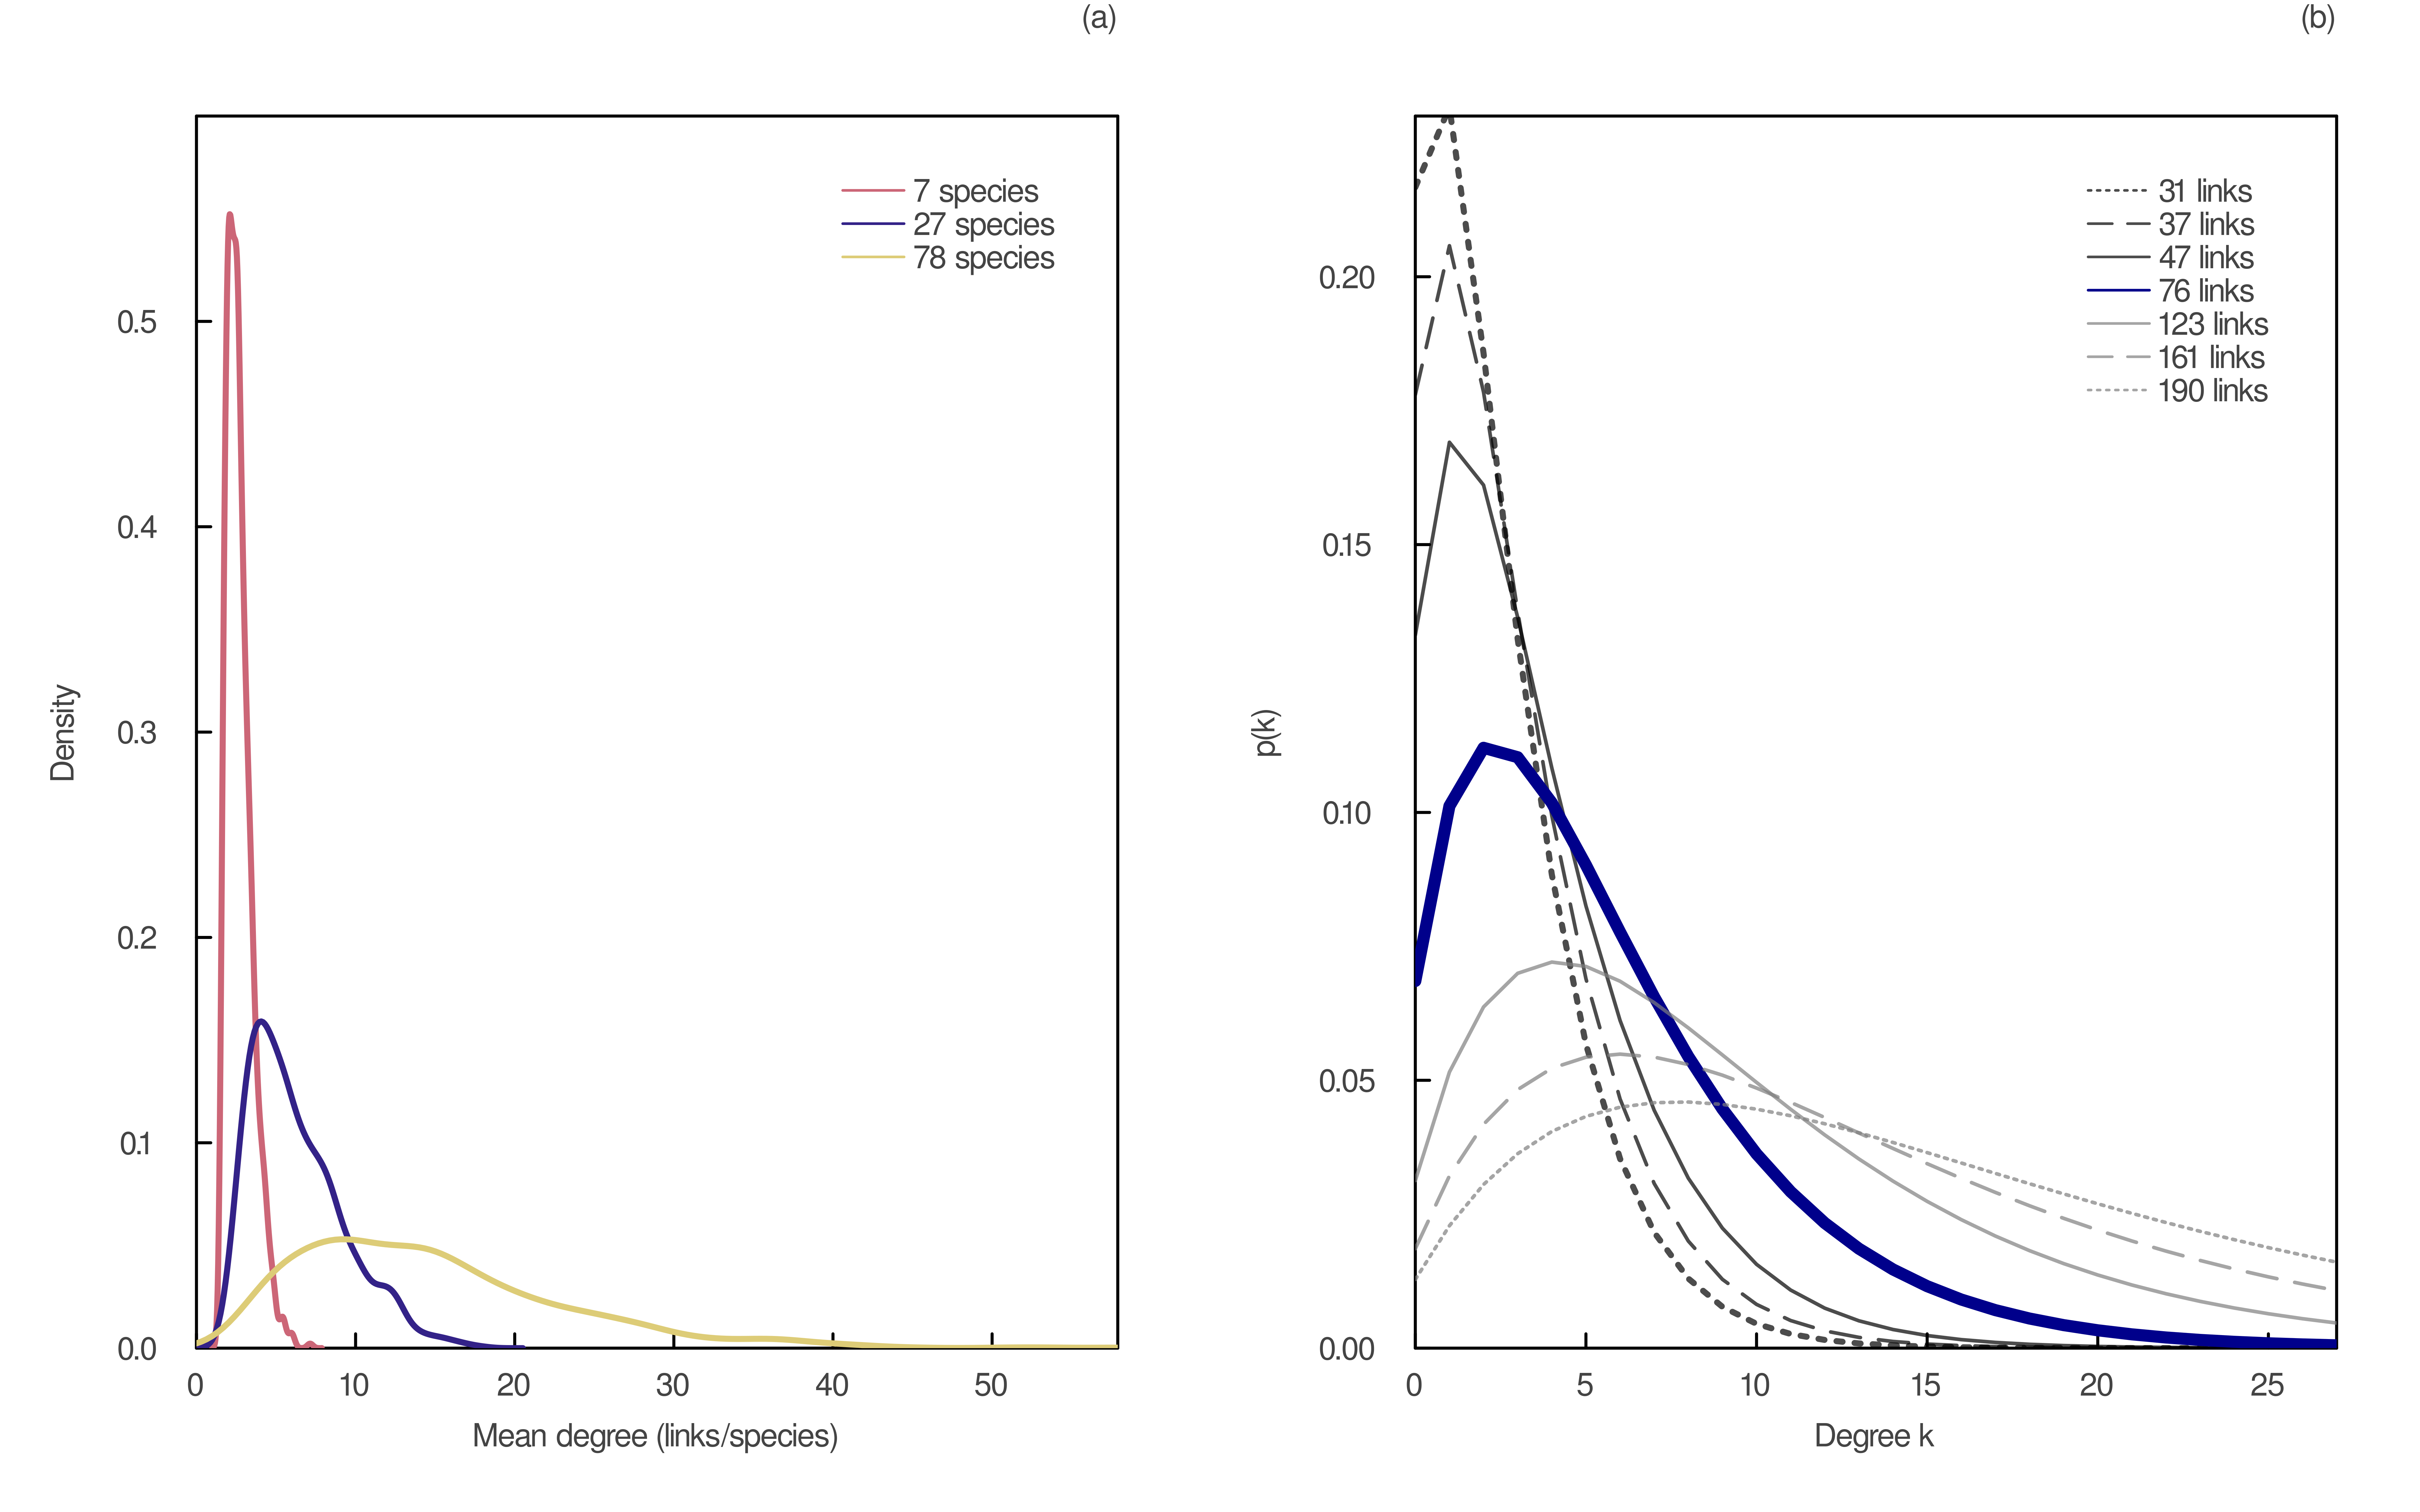
\includegraphics[width=\textwidth]{figures/article2/maxent_degree_dist_fl.png}
  \caption{\textbf{Maximum entropy degree distributions with predicted numbers of interactions.}
  (a) Probability density of the mean degree of a food web obtained using
  different values of species richness $S$. The number of interactions $L$ was
  simulated $1000$ times using the flexible links model fitted to all empirical
  networks. The mean degrees $2L/S$ were then obtained
  from these simulated values. (b) Degree distributions of maximum entropy for a
  network of $S=27$ species and different numbers of interactions. The numbers
  of interactions correspond to the lower and upper bounds of the $67\%$,
  $89\%$, and $97\%$ percentile intervals (PI), as well as the median (in blue),
  of the counterfactuals of the flexible links model. Each degree distribution
  of maximum entropy was obtained using Eq~\ref{eq:lagrange_dd} after solving
  numerically Eq~\ref{eq:lagrange2_dd} using different values of the mean
  degree constraint.}
  \label{fig:degree_dist_fl}
\end{figure}

\clearpage


\addcontentsline{toc}{section}{Box 3.2: Corresponding null and neutral models}

\newtcolorbox{box3.2}{colback=green!10,enhanced,title=Box \customlabel{box3.2}{3.2}: Corresponding null and neutral models,
	attach boxed title to top left={xshift=-4mm},boxrule=0pt,after skip=1cm,before skip=1cm,right skip=0cm,breakable,fonttitle=\bfseries,toprule=0pt,bottomrule=0pt,rightrule=0pt,leftrule=4pt,arc=0mm,skin=enhancedlast jigsaw,sharp corners,colframe=gree,colbacktitle=gre,boxed title style={
		frame code={ 
			\fill[gre](frame.south west)--(frame.north west)--(frame.north east)--([xshift=3mm]frame.east)--(frame.south east)--cycle;
			\draw[line width=1mm,gre]([xshift=2mm]frame.north east)--([xshift=5mm]frame.east)--([xshift=2mm]frame.south east);
			
			\draw[line width=1mm,gre]([xshift=5mm]frame.north east)--([xshift=8mm]frame.east)--([xshift=5mm]frame.south east);
			\fill[green!40](frame.south west)--+(4mm,-2mm)--+(4mm,2mm)--cycle;
		}
	}
}

\begin{box3.2}

\textbf{Null models (types I and II)}

The predictions of our heuristic maximum entropy models were compared against
two topological null models. These null models use the same ecological
information as our heuristic models and thus constitute an adequate baseline for
comparison. The first is the type I null model of \textcite{Fortuna2006Habitat}, in
which the probability that a species $i$ predates on another species $j$ is
given by
  
\begin{eqnarray}
\label{eq:type1null}
    p(i \rightarrow j) = \frac{L}{S^2}.
\end{eqnarray}
  
The second is the type II null model of \textcite{Bascompte2003Nested}, in which
the probability of interaction is instead given by 
  
\begin{eqnarray}
\label{eq:type2null}
    p(i \rightarrow j) = \frac{1}{2} \left(\frac{k_{in}(j)}{S} +
    \frac{k_{out}(i)}{S}\right),
\end{eqnarray}
  
where $k_{in}(j)$ and $k_{out}(i)$ are the in and out-degrees of species $j$ and
$i$, respectively. The type I null model is based on connectance, whereas the
type II null model is based on the joint degree sequence. Therefore, the type I
and II topological null models correspond to our type I and II heuristic MaxEnt
models, respectively, since they use similar constraints. 
  
We generated probabilistic networks using both types of null models for all
empirical food webs in our complete dataset. Then, we converted these networks
to adjacency matrices of Boolean values by generating $100$ random networks for
each of these probabilistic webs and kept the $L$ entries that were sampled the
most amount of times, with $L$ given by the number of interactions in each food
web. This ensured that the resulting null networks had the same number of
interactions as their empirical counterparts. Thus, for each null model, we
ended up with one null adjacency matrix for each empirical network. \\

\textbf{Neutral model}
  
We also compared our heuristic MaxEnt models to a neutral model of relative
abundances, in which the probabilities of interaction are given by
  
\begin{eqnarray}
\label{eq:neutralmodel}
    p(i \rightarrow j) \propto \frac{n_i}{N} \times \frac{n_j}{N},
\end{eqnarray}
  
where $n_i$ and $n_j$ are the abundances (or biomass) of both species and $N$ is
the total abundance (or biomass) of all species in the network. We generated
neutral abundance matrices for all empirical food webs in our abundance dataset
and converted these weighted networks to adjacency matrices of Boolean values
using the same method as the one we used for our null models. 

\end{box3.2}

\section{Results and Discussion}

\subsection{Analytical maximum entropy models}

We first discuss the predictive capacity of our analytical models. The
relationship between the relative numbers of prey $k_{out}$ and predators
$k_{in}$ in empirical networks and obtained from the joint degree distributions
of maximum entropy is depicted in the left and central panels of
Figure~\ref{fig:joint_dd}, respectively. We observe that our analytical model predicts
higher values of generality and vulnerability compared to empirical food webs
(i.e. relative values of $k_{out}$ and $k_{in}$ both closer to $1$) for many
species. In other words, our model predicts that species that have many
predators also have more prey than what is observed empirically (and
conversely). This is not surprising, given that our model did not include
biological factors preventing generalist predators from having many prey.
Nevertheless, with the exception of these generalist species, MaxEnt adequately
predicts that most species have low generality and vulnerability values.

\afterpage{\clearpage

\begin{figure}[!h]
  \centering
  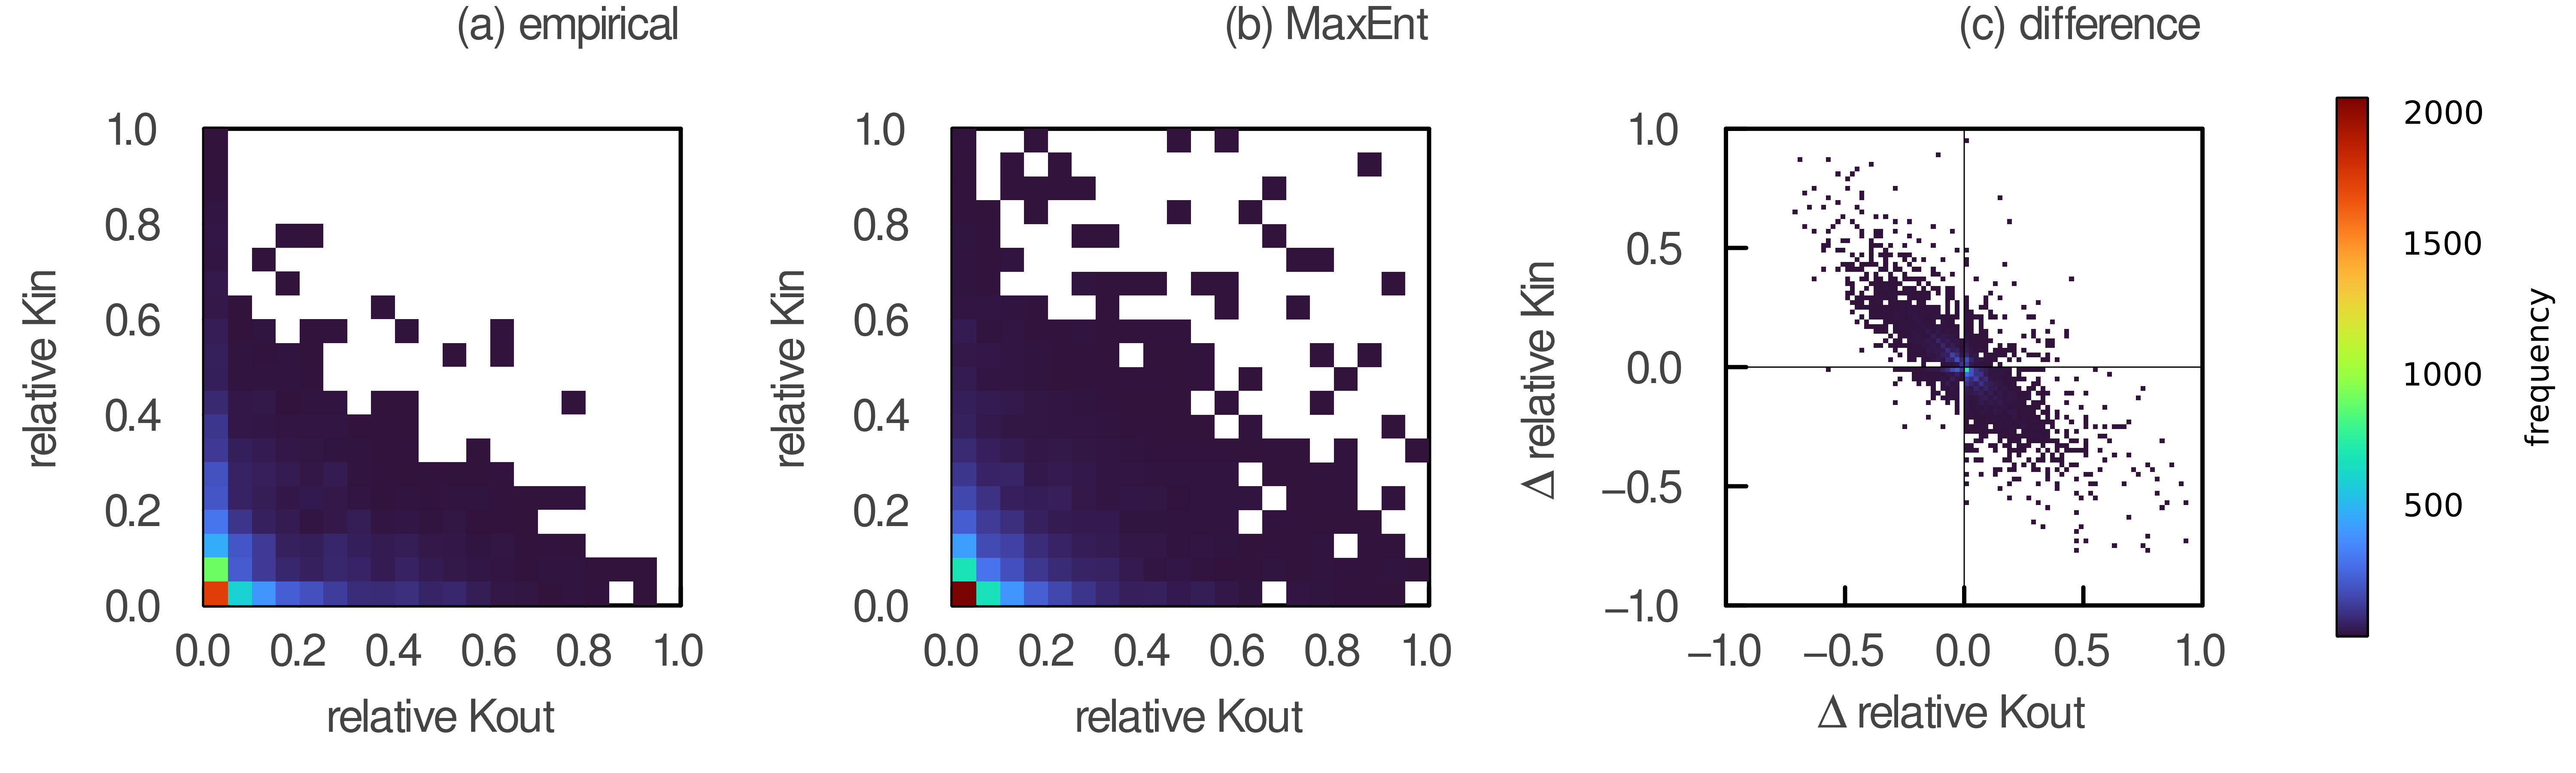
\includegraphics[width=\textwidth]{figures/article2/joint_degree_dist.png}
  \caption{\textbf{Prediction errors of the relative number of predators and prey.}
  The relative number of predators ($k_{in}$) is plotted against the relative
  number of prey ($k_{out}$) for each species in all (a) empirical and (b)
  predicted joint degree sequences. The predicted joint degree sequences were
  obtained after sampling one realization of the joint degree distribution of
  maximum entropy for each network while keeping the total number of
  interactions constant. (c) Difference between predicted and empirical values
  when species are ordered according to their total degree. Due to significant
  data overlap, all relationships are represented as 2D histograms. The color
  bar indicates the number of species that fall within each bin.}
\label{fig:joint_dd}
\end{figure}

}

Examining the difference between predicted and empirical values for each species
gives a slightly different perspective (right panel of Figure~\ref{fig:joint_dd}).
To make that comparison, we must first associate each of our predictions with a
specific species in a network. Indeed, our predicted joint degree sequences have
the same number of species (elements) as their empirical counterparts, but they
are species agnostic. In other words, instead of predicting a pair of values for
each species directly (i.e. the number of prey and predators of a given species
$i$), we predicted the entire joint degree sequence without taking into account
species' identity (i.e. the distribution of the number of prey and predators for
the entire set of species, without knowing which values belong to which
species). The challenge is thus to adequately associate predictions with
empirical data. In Figure~\ref{fig:joint_dd}, we present these differences when
species are ordered by their total degree in their respective networks (i.e. by
the sum of their in and out-degrees). This means that the species with the
highest total degree in its network will be associated with the highest
prediction, and so forth. Doing so, we see that species predicted to have a
higher number of predators than what is observed generally have a lower number
of prey than what is observed (and conversely). This is also shown in
Figure~\ref{fig:kin_kout_diff_strata} (Appendix~\ref{supp:B}), which represents the
relationship between prediction errors in the \textit{absolute} (non-relative)
values of $k_{out}$ and $k_{in}$ across networks of varying levels of species
richness. This is because the difference in total degree ($k_{out} + k_{in}$)
between predictions and empirical data is minimized when species are ranked by
their total degree (i.e. the average deviation of the sum of relative $k_{out}$
and $k_{in}$ is close to $0$ across all species). This result thus shows that
the difference between predicted and empirical total degrees is low for most
species when ordered by their total degrees. There are no apparent biases
towards in or out degrees. In Figure~\ref{fig:kin_kout_diff}
(Appendix~\ref{supp:B}), we show how these differences change when species are
instead ordered by their out-degrees (left panel) and in-degrees (right panel),
i.e. when minimizing the error in the estimation of the out and in-degrees,
respectively.

Another way to evaluate the empirical support of the sampled joint degree
sequences is to compare their shape with the ones of empirical food webs. We
described the shape of a joint degree sequence by measuring the distance between
its in and out-degree sequences (i.e. the distance between its marginal
distributions). To do so, we calculated the Kullback–Leibler (KL) divergence
(\cite{Kullback1951Information}) between the in and out-degree sequences of each
predicted and empirical distribution. The KL divergence is a measure of relative
entropy describing the difference between two distributions. Low values indicate
high similarity between the in and out-degree sequences and suggest that the
joint degree sequence has a high level of symmetry. We compared the shape of the
empirical and predicted joint degree sequences in the left panel of
Figure~\ref{fig:kl_diverg}. As expected, our model predicts more similar in-degree and
out-degree sequences than empirical data (shown by lower KL divergence values).
However, the difference between the KL divergence of predicted and empirical
joint degree sequences decreases with connectance (right panel of
Figure~\ref{fig:kl_diverg}). This might be because food webs with a low connectance are
harder to predict than food webs with a high connectance. Indeed, in low
connectance systems, what makes two species interact may be more important for
prediction than in high connectance systems, in which what prevents species from
interacting may be more meaningful. This implies that more ecological
information may be needed in food webs with a low connectance because more
ecological processes determine interactions compared to non-interactions.
Therefore, other ecological constraints might be needed to account for the
asymmetry of the joint degree distribution, especially for networks with a lower
connectance. Nevertheless, our MaxEnt model seems to capture quite well the
shape of the joint degree sequence for networks having a high connectance.

\afterpage{\clearpage

\begin{figure}[!h]
  \centering
  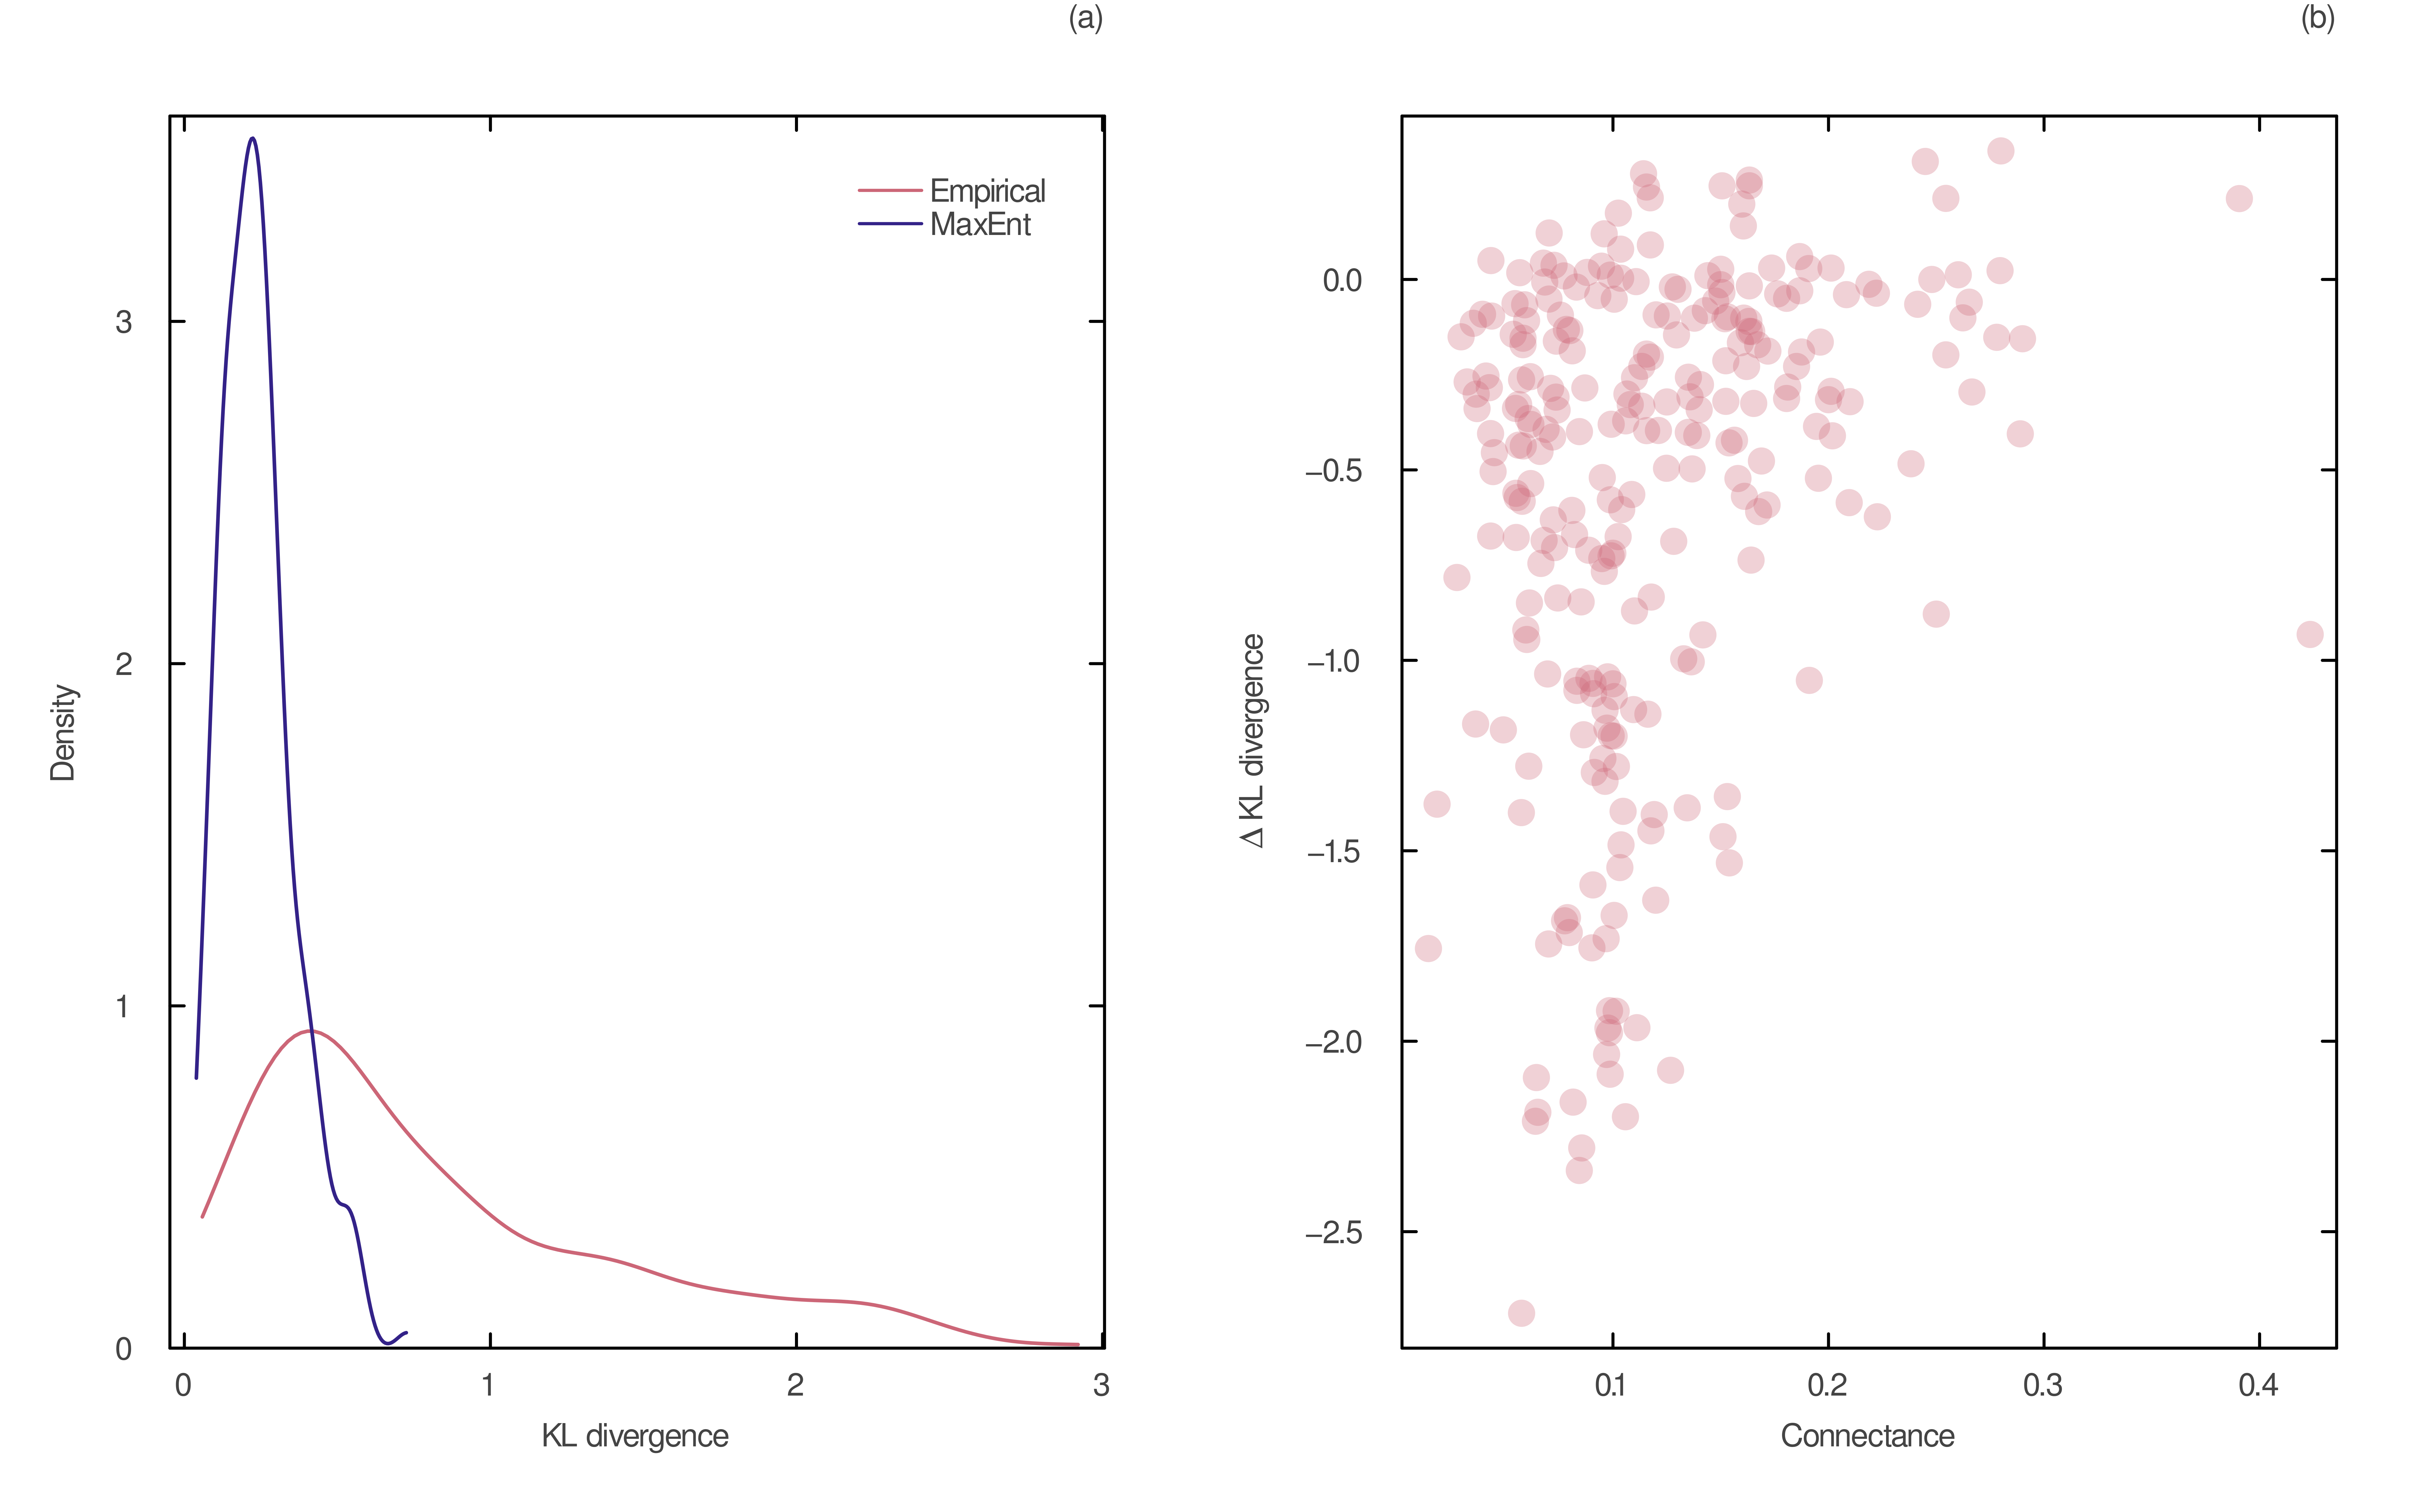
\includegraphics[width=\textwidth]{figures/article2/kl_divergence.png}
  \caption{\textbf{Shape of empirical and predicted joint degree sequences.}
  (a) Probability density of KL divergence between in and out-degree sequences of
  empirical and predicted joint degree sequences. (b) Difference between the KL
  divergence of empirical and predicted joint degree sequences as a function of
  connectance. The predicted joint degree sequences were obtained after sampling
  one realization of the joint degree distribution of maximum entropy for each
  network while keeping the total number of interactions constant.}
\label{fig:kl_diverg}
\end{figure}

}

Regarding the degree distribution of maximum entropy, one aspect that informs us
of its ecological realism is the number of isolated species it predicts. As
\textcite{MacDonald2020Revisiting} pointed out, the size of food webs should at
least be of $S-1$ interactions since a lower number would yield isolated
species, i.e. species without any predator or prey. Because non-basal species
must eat to survive, isolated species could indicate that other species are
missing; otherwise, isolated species should be removed from the network. In
Figure~\ref{fig:heatmap} (Appendix~\ref{supp:B}), we show that the degree
distribution of maximum entropy, given $S$ and $L$, gives a very low probability
that a species will be isolated in its food web (i.e. having $k = 0$) when $L >
S-1$. However, under our purely information-theoretic model, the probability
that a species is isolated is quite high when the total number of interactions
is below $S-1$. Moreover, the expected proportion of isolated species rapidly
declines by orders of magnitude with increasing numbers of species and
interactions. This supports the ecological realism of the degree distribution of
maximum entropy derived above. Nevertheless, ecologists wanting to model a
system without allowing isolated species could simply change the lower limit of
$k$ to $1$ in Eq~\ref{eq:lagrange2_dd} and solve the resulting equation
numerically.

\subsection{Heuristic maximum entropy models}

In this section, we explore the predictions of our heuristic models. Overall, we
found that the models based on the joint degree sequence (i.e. the type II null
and heuristic MaxEnt models) reproduced the structure of empirical food webs
much better than the ones based on connectance (i.e. the type I null and
heuristic MaxEnt models, Table~\ref{tbl:measures_all}). This suggests that the
predictive capacity of connectance might be more limited than what was
previously suggested (\cite{Poisot2014When}). On the other hand, the neutral
model of relative abundances was surprisingly good at predicting the maximum
trophic level and the network diameter (Table~\ref{tbl:measures_abund}). However,
with the exception of the network diameter, the type II heuristic MaxEnt model
was better at predicting network structure than the neutral model for most
measures considered. This might be because, although neutral processes are
important, they act in concert with niche processes in determining species
interactions (\cite{Bartomeus2016Common}, \cite{Canard2014Empirical},
\cite{Poisot2015Species}, \cite{Pomeranz2019Inferring}). The joint degree sequence
captures information on both neutral and niche processes because the number of
prey and predators a species has is determined by its relative abundance and
biological traits. These results thus show that having information on the number
of prey and predators for each species substantially improves the prediction of
food-web structure, both compared to models solely based on connectance and to
the ones solely based on species relative abundances.

\afterpage{\clearpage

\begin{table}[!h]
  \resizebox{\textwidth}{!}{
  \centering
  \begin{tabular}{c c c c c c c c } 
   \hline
   {\bf model} & {\bf $\rho$} & {\bf maxtl} & {\bf diam} & {\bf MxSim} & {\bf
  Cannib} & {\bf Omniv} & {\bf entropy} \\
  \hline
  null 1 & -0.167 &  0.980 & 1.428 & -0.502 &  2.007 & 1.493 & 0.056 \\ 
  MaxEnt 1 & -0.226 & 0.831 & 1.274 & -0.524 & 1.982 & 1.863 & 0.106 \\ 
  null 2 & 0.160 & -0.125 & 0.016 & 0.007 & 1.078 & 0.559 & -0.023 \\ 
  MaxEnt 2 & -0.015 & 0.178 & 0.565 & -0.282 & 0.698 & 0.589 & 0.058 \\ 
  \hline
  \end{tabular}
  }
  \caption{\textbf{Standardized mean difference between predicted network measures
and empirical data for all food webs in our complete dataset ($N = 257$).} Positive (negative) values indicate that the measure is
overestimated (underestimated) on average. Null 1: Type I null model based on
connectance. MaxEnt 1: Type I heuristic MaxEnt model based on connectance.
Null 2: Type II null model based on the joint degree sequence. MaxEnt 2: Type
II heuristic MaxEnt model based on the joint degree sequence. $\rho$:
nestedness measured by the spectral radius of the adjacency matrix.
\textit{maxtl}: maximum trophic level. \textit{diam}: network diameter.
\textit{MxSim}: average maximum similarity between species pairs.
\textit{Cannib}: proportion of cannibal species (self-loops). \textit{Omniv}:
proportion of omnivorous species. \textit{entropy}: SVD entropy.}
  \label{tbl:measures_all}
\end{table}

\begin{table}[!b]
  \resizebox{\textwidth}{!}{
  \centering
  \begin{tabular}{c c c c c c c c } 
   \hline
   {\bf model} & {\bf $\rho$} & {\bf maxtl} & {\bf diam} & {\bf MxSim} & {\bf Cannib} & {\bf Omniv} & {\bf entropy} \\
  \hline
  neutral & 0.367 & -0.090 & 0.027 & 0.266 & 6.870 & 0.576 & -0.083 \\ 
  null 1 & -0.134 & 0.950 & 1.919 & -0.369 & 2.077 & 0.614 & 0.068 \\ 
  MaxEnt 1 & -0.229 & 1.020 & 1.946 & -0.355 & 2.215 & 0.801 & 0.121 \\ 
  null 2 & 0.128 & -0.115 & -0.135 & 0.157 & 1.444 & 0.029 & -0.021 \\ 
  MaxEnt 2 & -0.010 & 0.054 & 0.243 & -0.062 & -0.038 & 0.083 & 0.038 \\ 
  \hline
  \end{tabular}
  }
  \caption{\textbf{Standardized mean difference between predicted network measures and empirical data for all food webs in our abundance dataset ($N = 19$).} Positive (negative) values indicate that the measure is
overestimated (underestimated) on average. Null 1: Type I null model based on
connectance. MaxEnt 1: Type I heuristic MaxEnt model based on connectance.
Null 2: Type II null model based on the joint degree sequence. MaxEnt 2: Type
II heuristic MaxEnt model based on the joint degree sequence. $\rho$:
nestedness measured by the spectral radius of the adjacency matrix.
\textit{maxtl}: maximum trophic level. \textit{diam}: network diameter.
\textit{MxSim}: average maximum similarity between species pairs.
\textit{Cannib}: proportion of cannibal species (self-loops). \textit{Omniv}:
proportion of omnivorous species. \textit{entropy}: SVD entropy.}
  \label{tbl:measures_abund}
\end{table}

\clearpage
}

Next, the predictions of the type II heuristic MaxEnt model can be compared to
its null model counterpart. On average, the type II heuristic MaxEnt model was
better at predicting nestedness ($0.62 \pm 0.08$) than its corresponding null
model ($0.73 \pm 0.05$; empirical networks: $0.63 \pm 0.09$) for networks in our
complete dataset (Table~\ref{tbl:measures_all}). This might in part be due to the
fact that nestedness was calculated using the spectral radius of the adjacency
matrix, which directly leverages information on the network itself just like the
heuristic MaxEnt model. The proportion of self-loops (cannibal species) was also
better predicted by the type II heuristic MaxEnt model in comparison to the type
II null model. However, the type II null model was better at predicting network
diameter and average maximum similarity between species pairs, and predictions
of the maximum trophic level and the proportion of omnivorous species were
similar between both types of models. We believe that this is because increasing
the complexity of a food web might increase its average and maximum food-chain
lengths. In comparison, the null model was more stochastic and does not
necessarily produce more complex food webs with longer food-chain lengths. 

Moreover, we found that the entropy of empirical food webs was slightly lower
than their maximum entropy when constrained by their joint degree sequence
Figure~\ref{fig:entropy_dist} (Appendix~\ref{supp:B}). Empirical food webs had an
SVD entropy of $0.89 \pm 0.04$, compared to an SVD entropy of $0.94 \pm 0.03$
for networks generated using the type II heuristic MaxEnt model. The
relationship between the SVD entropy of empirical food webs and their maximum
entropy is plotted in the last panel of Figure~\ref{fig:measures}. The slight
increase in entropy confirms that our method generated more complex networks.
Even though we found that many measures of empirical networks are close to the
ones of their maximum entropy configuration, the relatively low predictability
of entropy itself may be indicative of additional constraints shaping food-web
structure, especially for networks with low SVD entropy. Incorporating more
constraints into the model could increase its capacity to generate networks with
an adequate level of complexity, as shown by the decrease in predictive errors
of entropy of the type II heuristic MaxEnt model compared to the one based on
connectance (Table~\ref{tbl:measures_all}). Additionally, we found no clear
relationship between the increase in SVD entropy and the number of species, the
number of interactions, and connectance Figure~\ref{fig:entropy_size}
(Appendix~\ref{supp:B}). This suggests that our model captured the complexity of
small and large networks on a similar level and that its capacity to reproduce
food-web structure was unrelated to the order and size of the network. In other
words, the gap in entropy between empirical food webs and their maximum entropy
configuration may be the result of additional constraints that were not taken
into account in the model, regardless of the number of species and the number of
interactions. 

\afterpage{\clearpage

\begin{figure}[!h]
  \centering
  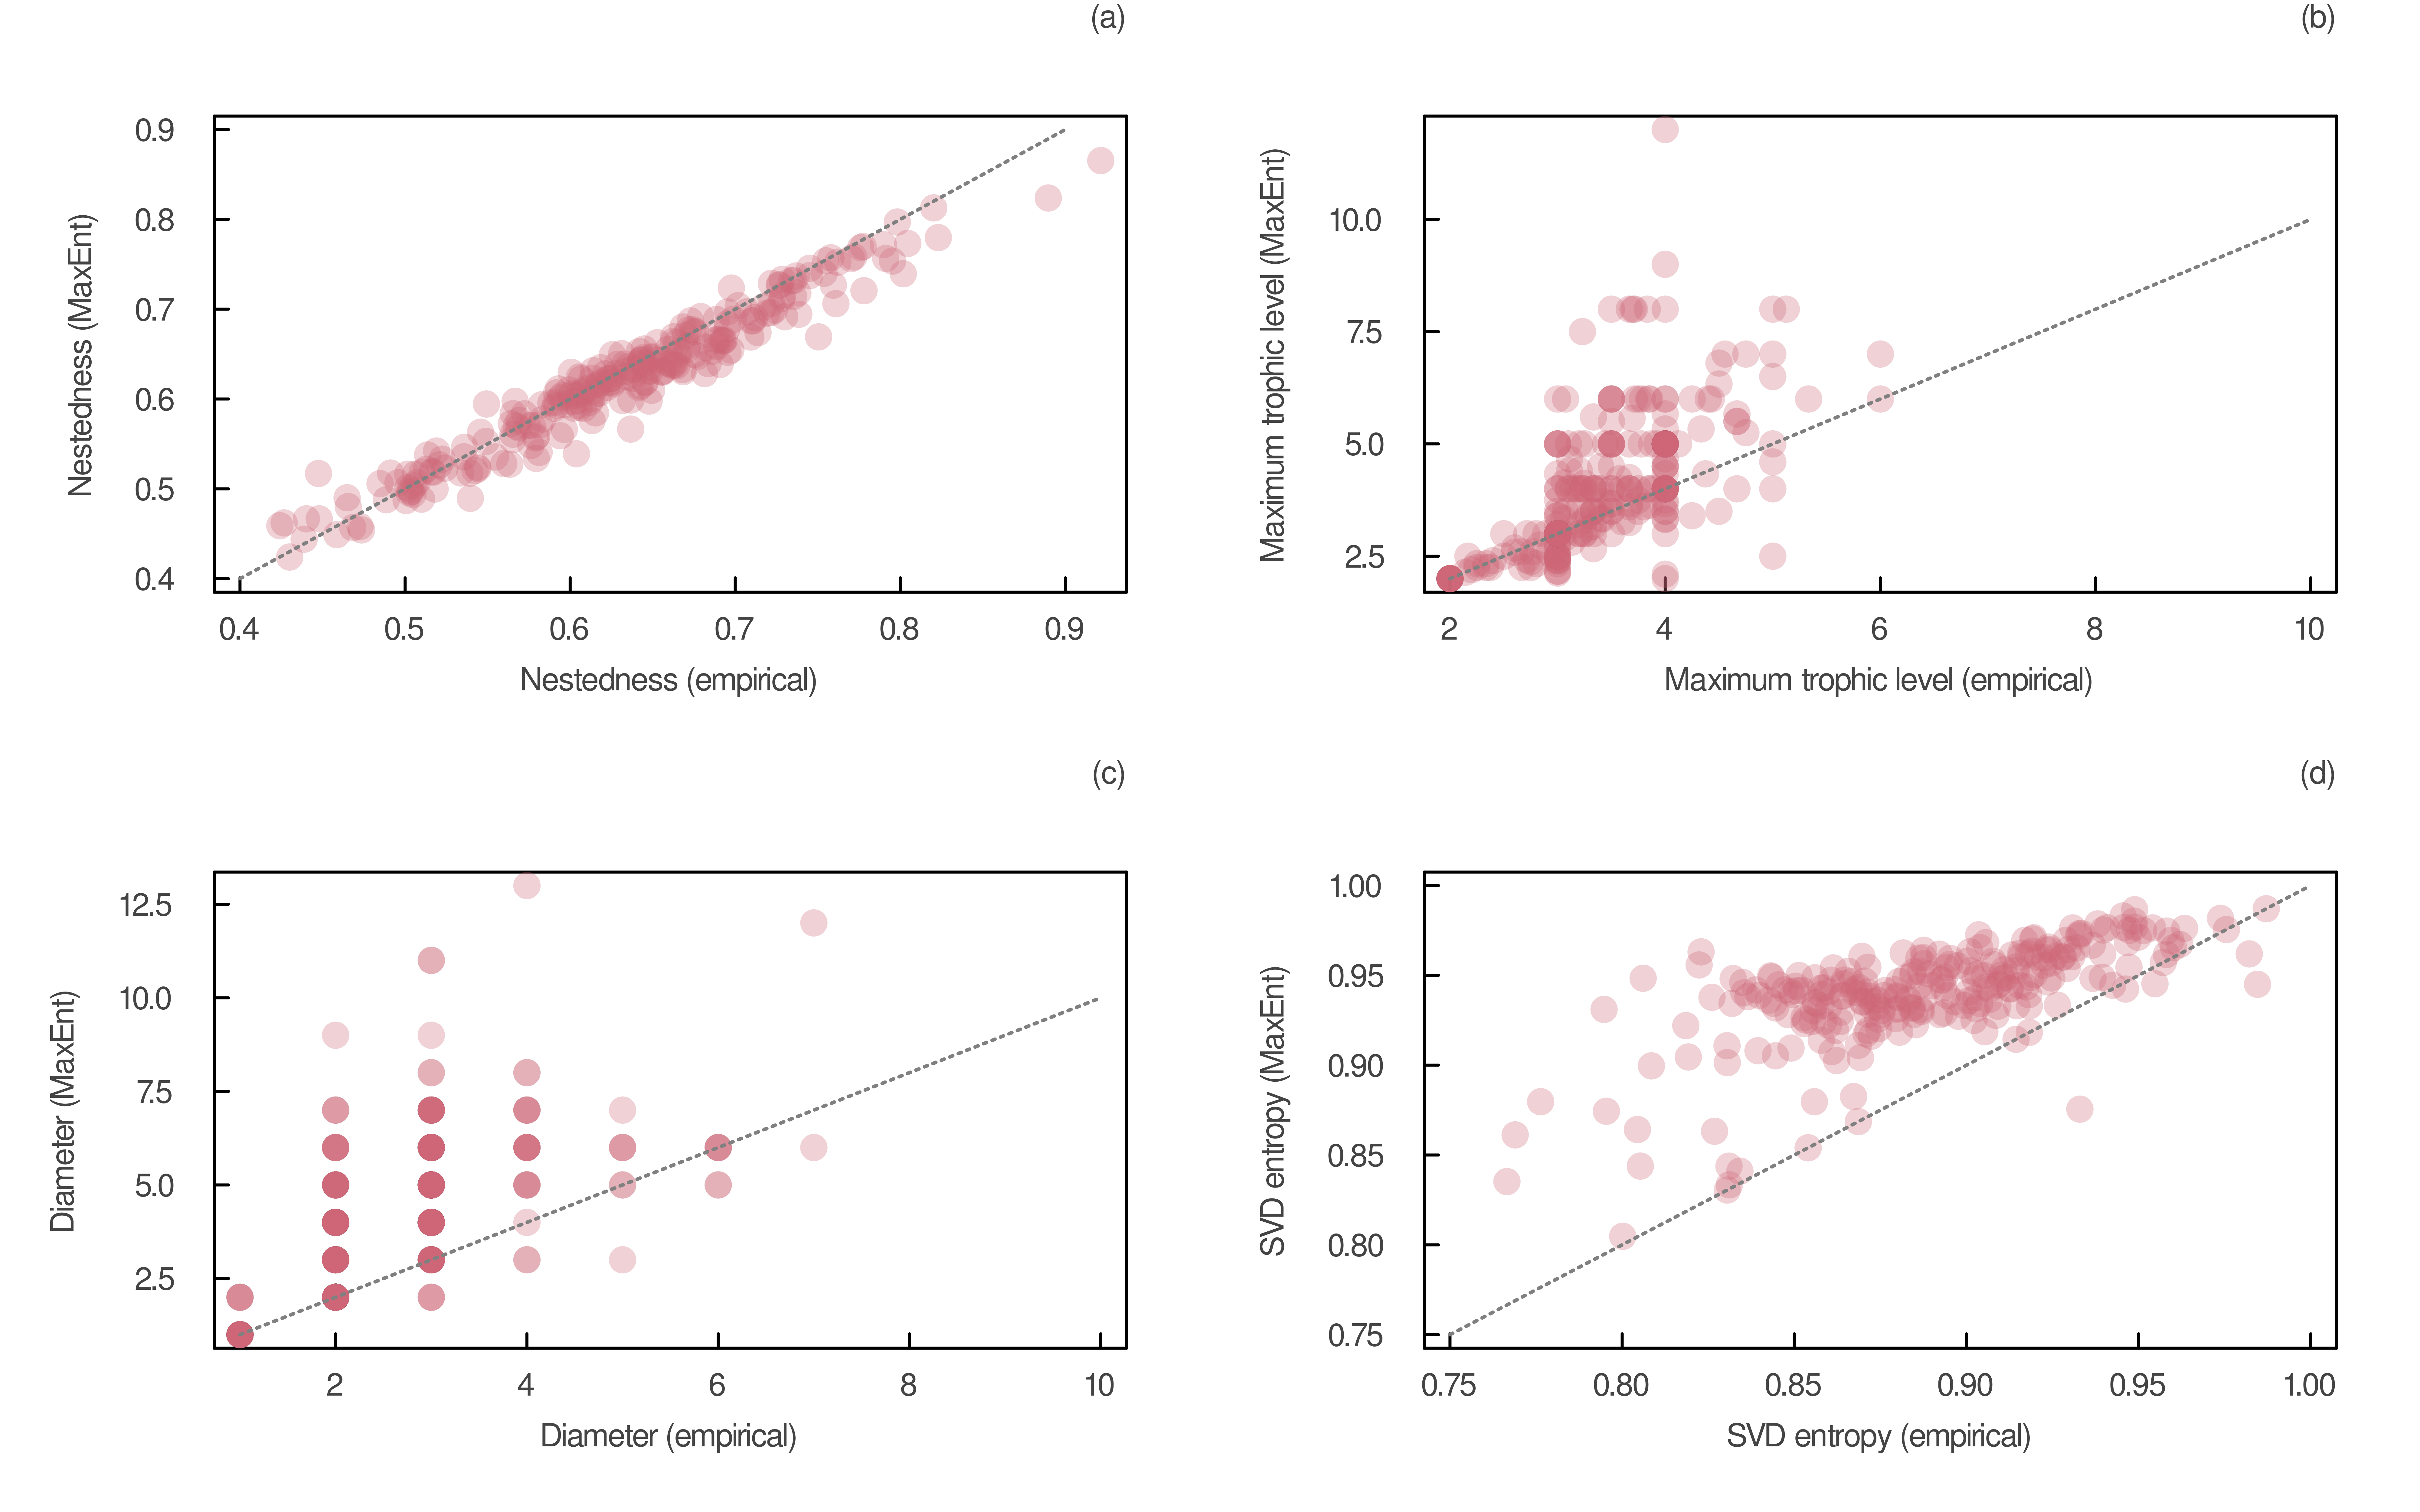
\includegraphics[width=\textwidth]{figures/article2/measures_emp_maxent.png}
  \caption{\textbf{Relationship between the structure of empirical and maximum entropy food webs.}
  Maximum entropy networks were obtained using the type II heuristic MaxEnt
  model based on the joint degree sequence. (a) Nestedness (estimated using the
  spectral radius of the adjacency matrix), (b) the maximum trophic level, (c)
  the network diameter, and (d) the SVD entropy were measured on these empirical
  and maximum entropy food webs. The identity line is plotted in each panel.}
  \label{fig:measures}
\end{figure}

}

A direct comparison of the structure of maximum entropy food webs constrained by
the joint degree sequence with empirical data also supports the results depicted
in Table~\ref{tbl:measures_all}. In Figure~\ref{fig:measures}, we show how well
empirical measures are predicted by the type II heuristic MaxEnt model.
Following our previous results, we found that nestedness was very well predicted
by our model. However, the model overestimated the maximum trophic level and
network diameter, especially when the sampled food web had intermediate values
of these measures. In Figure~\ref{fig:measures_richness} (Appendix~\ref{supp:B}),
we show that the pairwise relationships between the four measures in
Figure~\ref{fig:measures} and species richness in empirical food webs are similar
(in magnitude and sign) to the ones found in food webs generated using the type
II heuristic MaxEnt model. This indicates that the number of species in the
network does not seem to impact the ability of the model to reproduce food-web
structure. 

Notwithstanding its difficulties in reproducing adequate measures of food-chain
lengths, the type II heuristic MaxEnt model can predict surprisingly well the
proportions of three-species motifs in empirical food webs. Motifs have been
shown to be the backbone of complex ecological networks on which network
structure is built and play a crucial role in community dynamics and assembly
(\cite{Stouffer2011Compartmentalization}). Differences in motif profiles between an observed
food web and null model-generated ones can unveil important ecological
mechanisms that contribute to network structure (\cite{Stouffer2007Evidence}). In
Figure~\ref{fig:motifs}, we show that the motif profile of networks generated using the
type II heuristic MaxEnt model accurately reproduced the one of empirical data.
This model made significantly better predictions than the ones based on
connectance and the type II null model based on the joint degree sequence. This
is also shown in Figure~\ref{fig:motifs_rel}, which reveals that the relationships
between the proportions of single-link motifs in empirical food webs are similar
to the ones in networks generated using the type II heuristic MaxEnt model. This
is in contrast with the type I null and MaxEnt models based on connectance,
which produced opposite relationships than what was observed empirically. Our
findings show that generating the most complex food web constrained by the joint
degree sequence using maximum entropy does not alter the proportions of
three-species motifs on the whole. This suggests that motif profiles may simply
be a statistical attribute of food webs driven by the joint degree sequence.
However, given the incapacity of our MaxEnt models to accurately predict
food-chain lengths, the way motifs interconnect with each other may hold greater
biological significance than the proportion of motifs itself. 

\afterpage{\clearpage

\begin{figure}[!h]
  \centering
  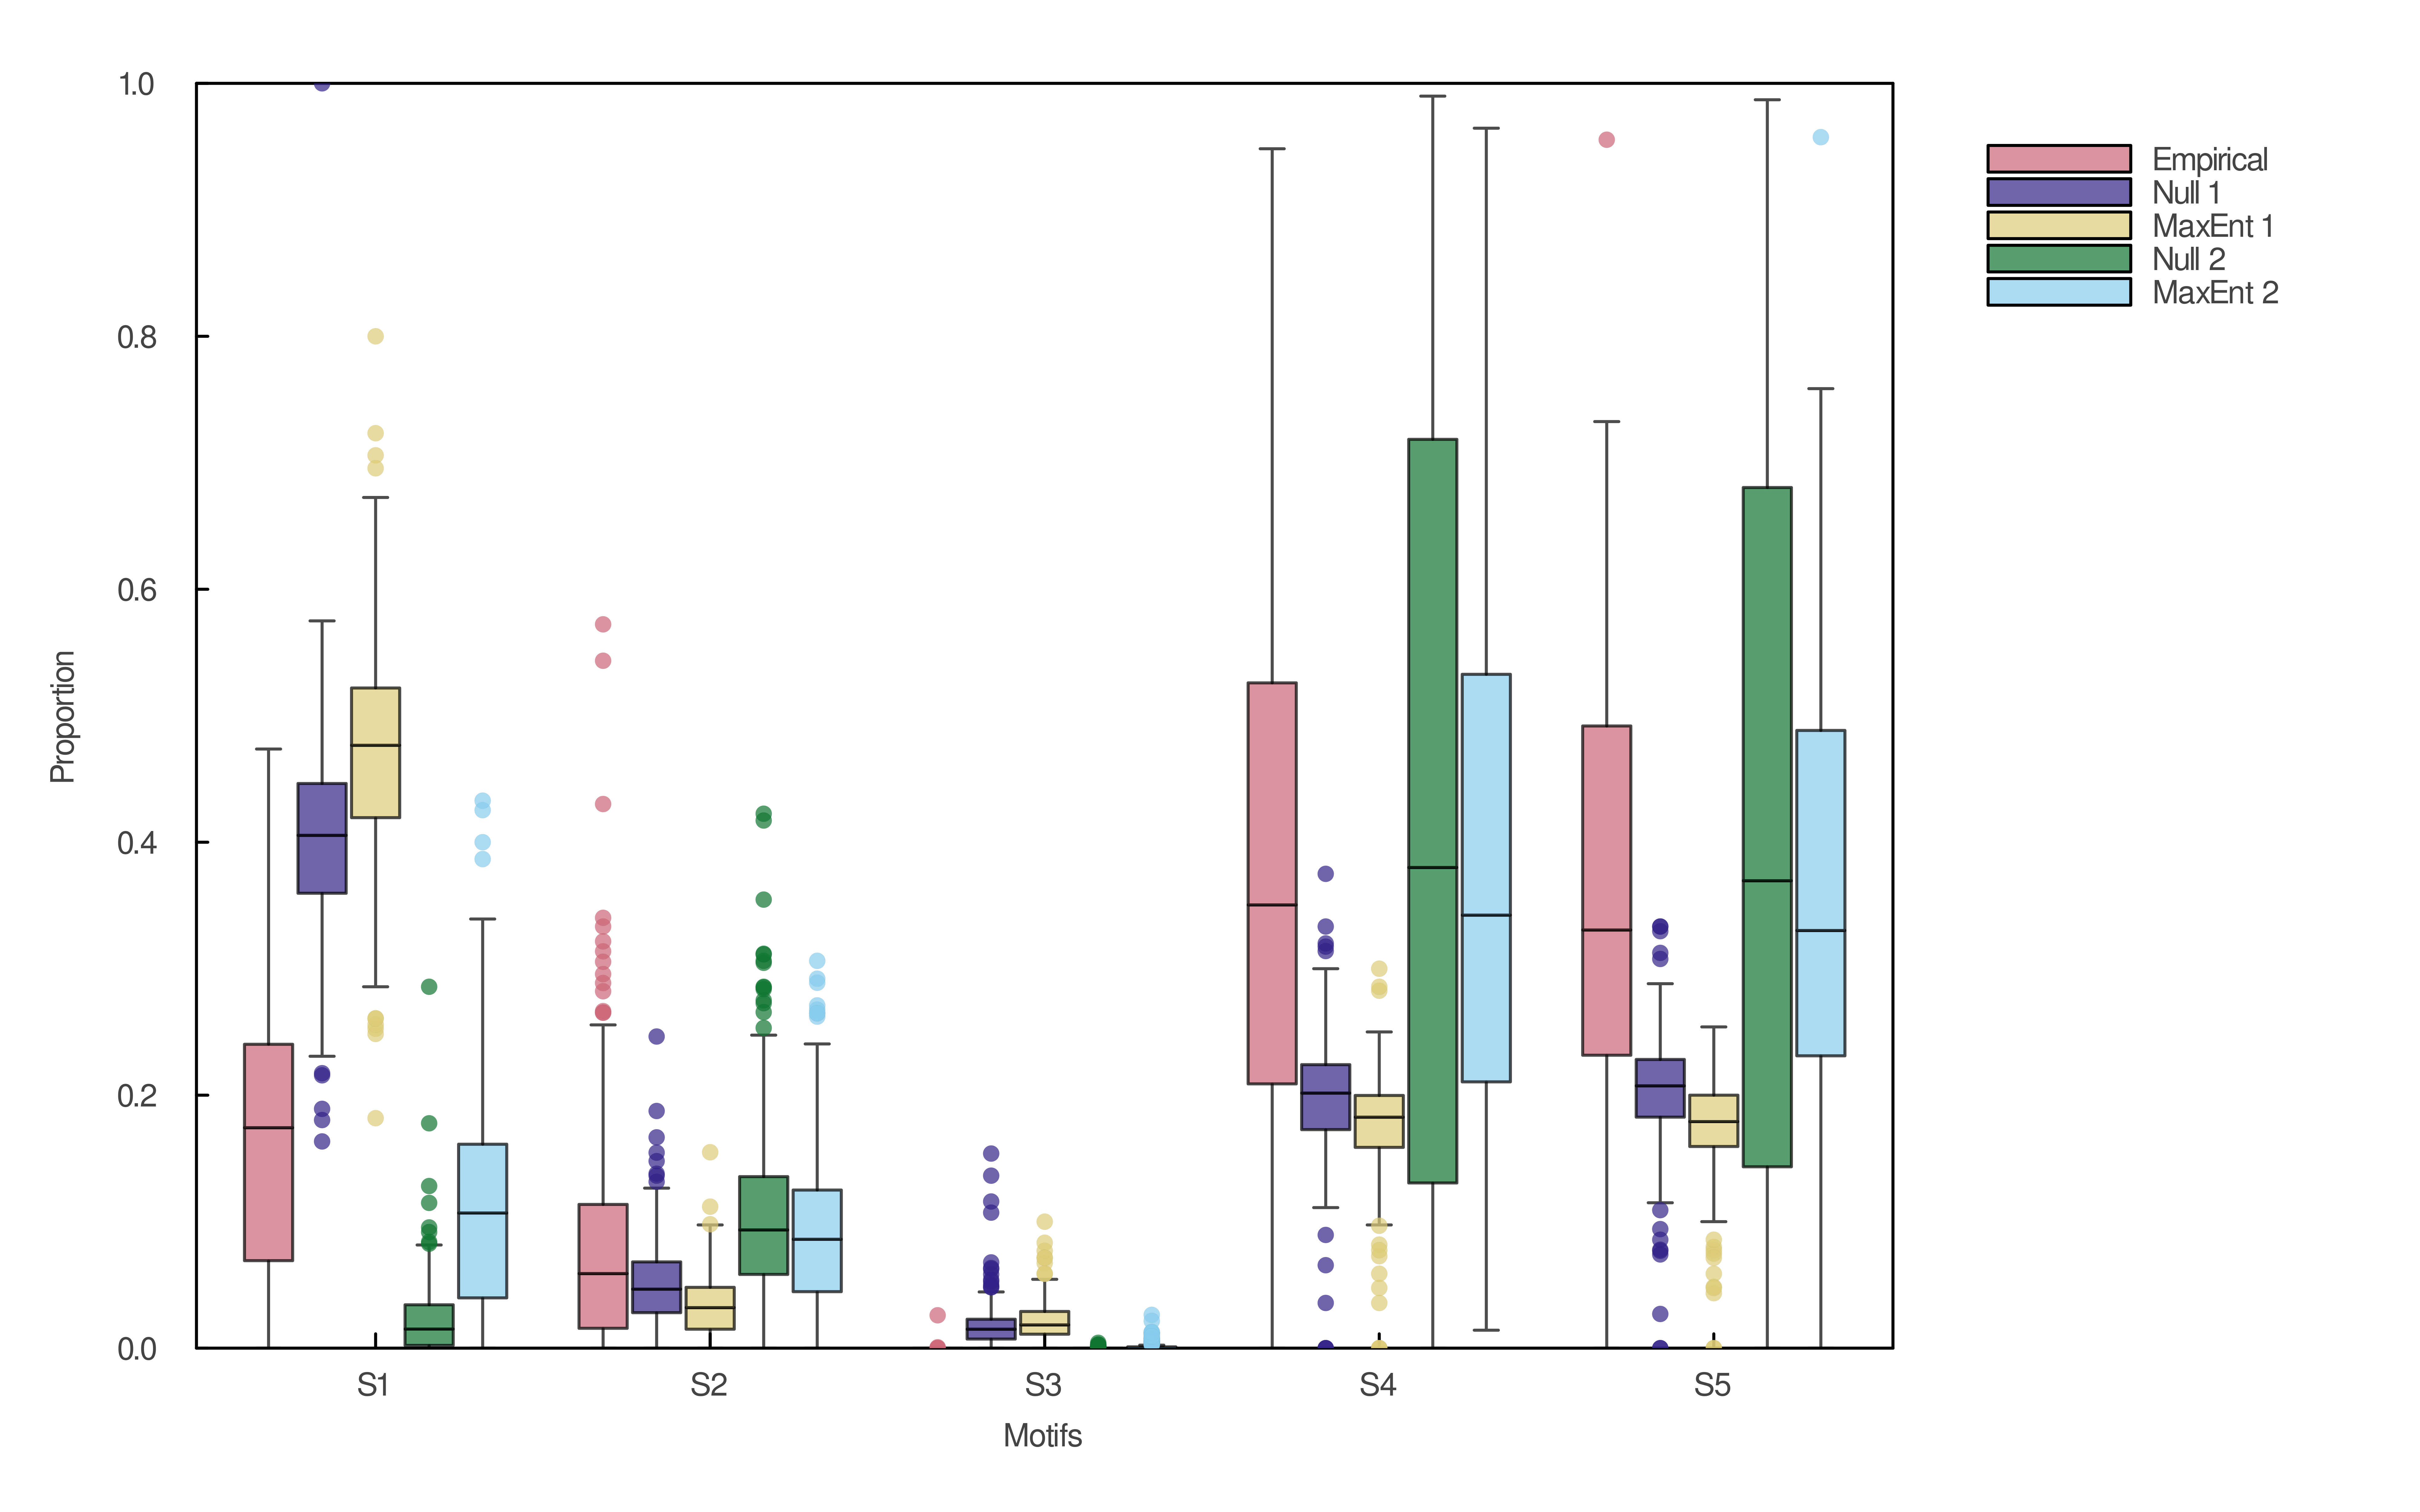
\includegraphics[width=\textwidth]{figures/article2/motifs_distribution.png}
  \caption{\textbf{Proportions of single-link three-species motifs in empirical and predicted food webs.}
  S1: Tri-trophic chain (a top predator feeds on a meso-predator which feeds on
  a basal prey). S2: Omnivory (a top predator feeds on a meso-predator and a
  basal prey). S3: Tri-trophic feeding loop (a cyclic three-species
  predator-prey system). S4: Apparent competition (a predator feeds on two
  prey). S5: Exploitative competition (two predators feed on the same prey).
  Null 1: Type I null model based on connectance. MaxEnt 1: Type I heuristic
  MaxEnt model based on connectance. Null 2: Type II null model based on the
  joint degree sequence. MaxEnt 2: Type II heuristic MaxEnt model based on the
  joint degree sequence. Boxplots display the median proportion of each motif in
  food webs (middle horizontal lines), as well as the first (bottom horizontal
  lines) and third (top horizontal lines) quartiles. Vertical lines encompass
  all data points that fall within $1.5$ times the interquartile range from both
  quartiles, and dots are data points that fall outside this range. Only the
  single-link motifs S1-S5 are shown given the scarcity of double-link motifs in
  most empirical and predicted networks. }
\label{fig:motifs}
\end{figure}

}

\afterpage{\clearpage

\begin{figure}[!h]
  \centering
  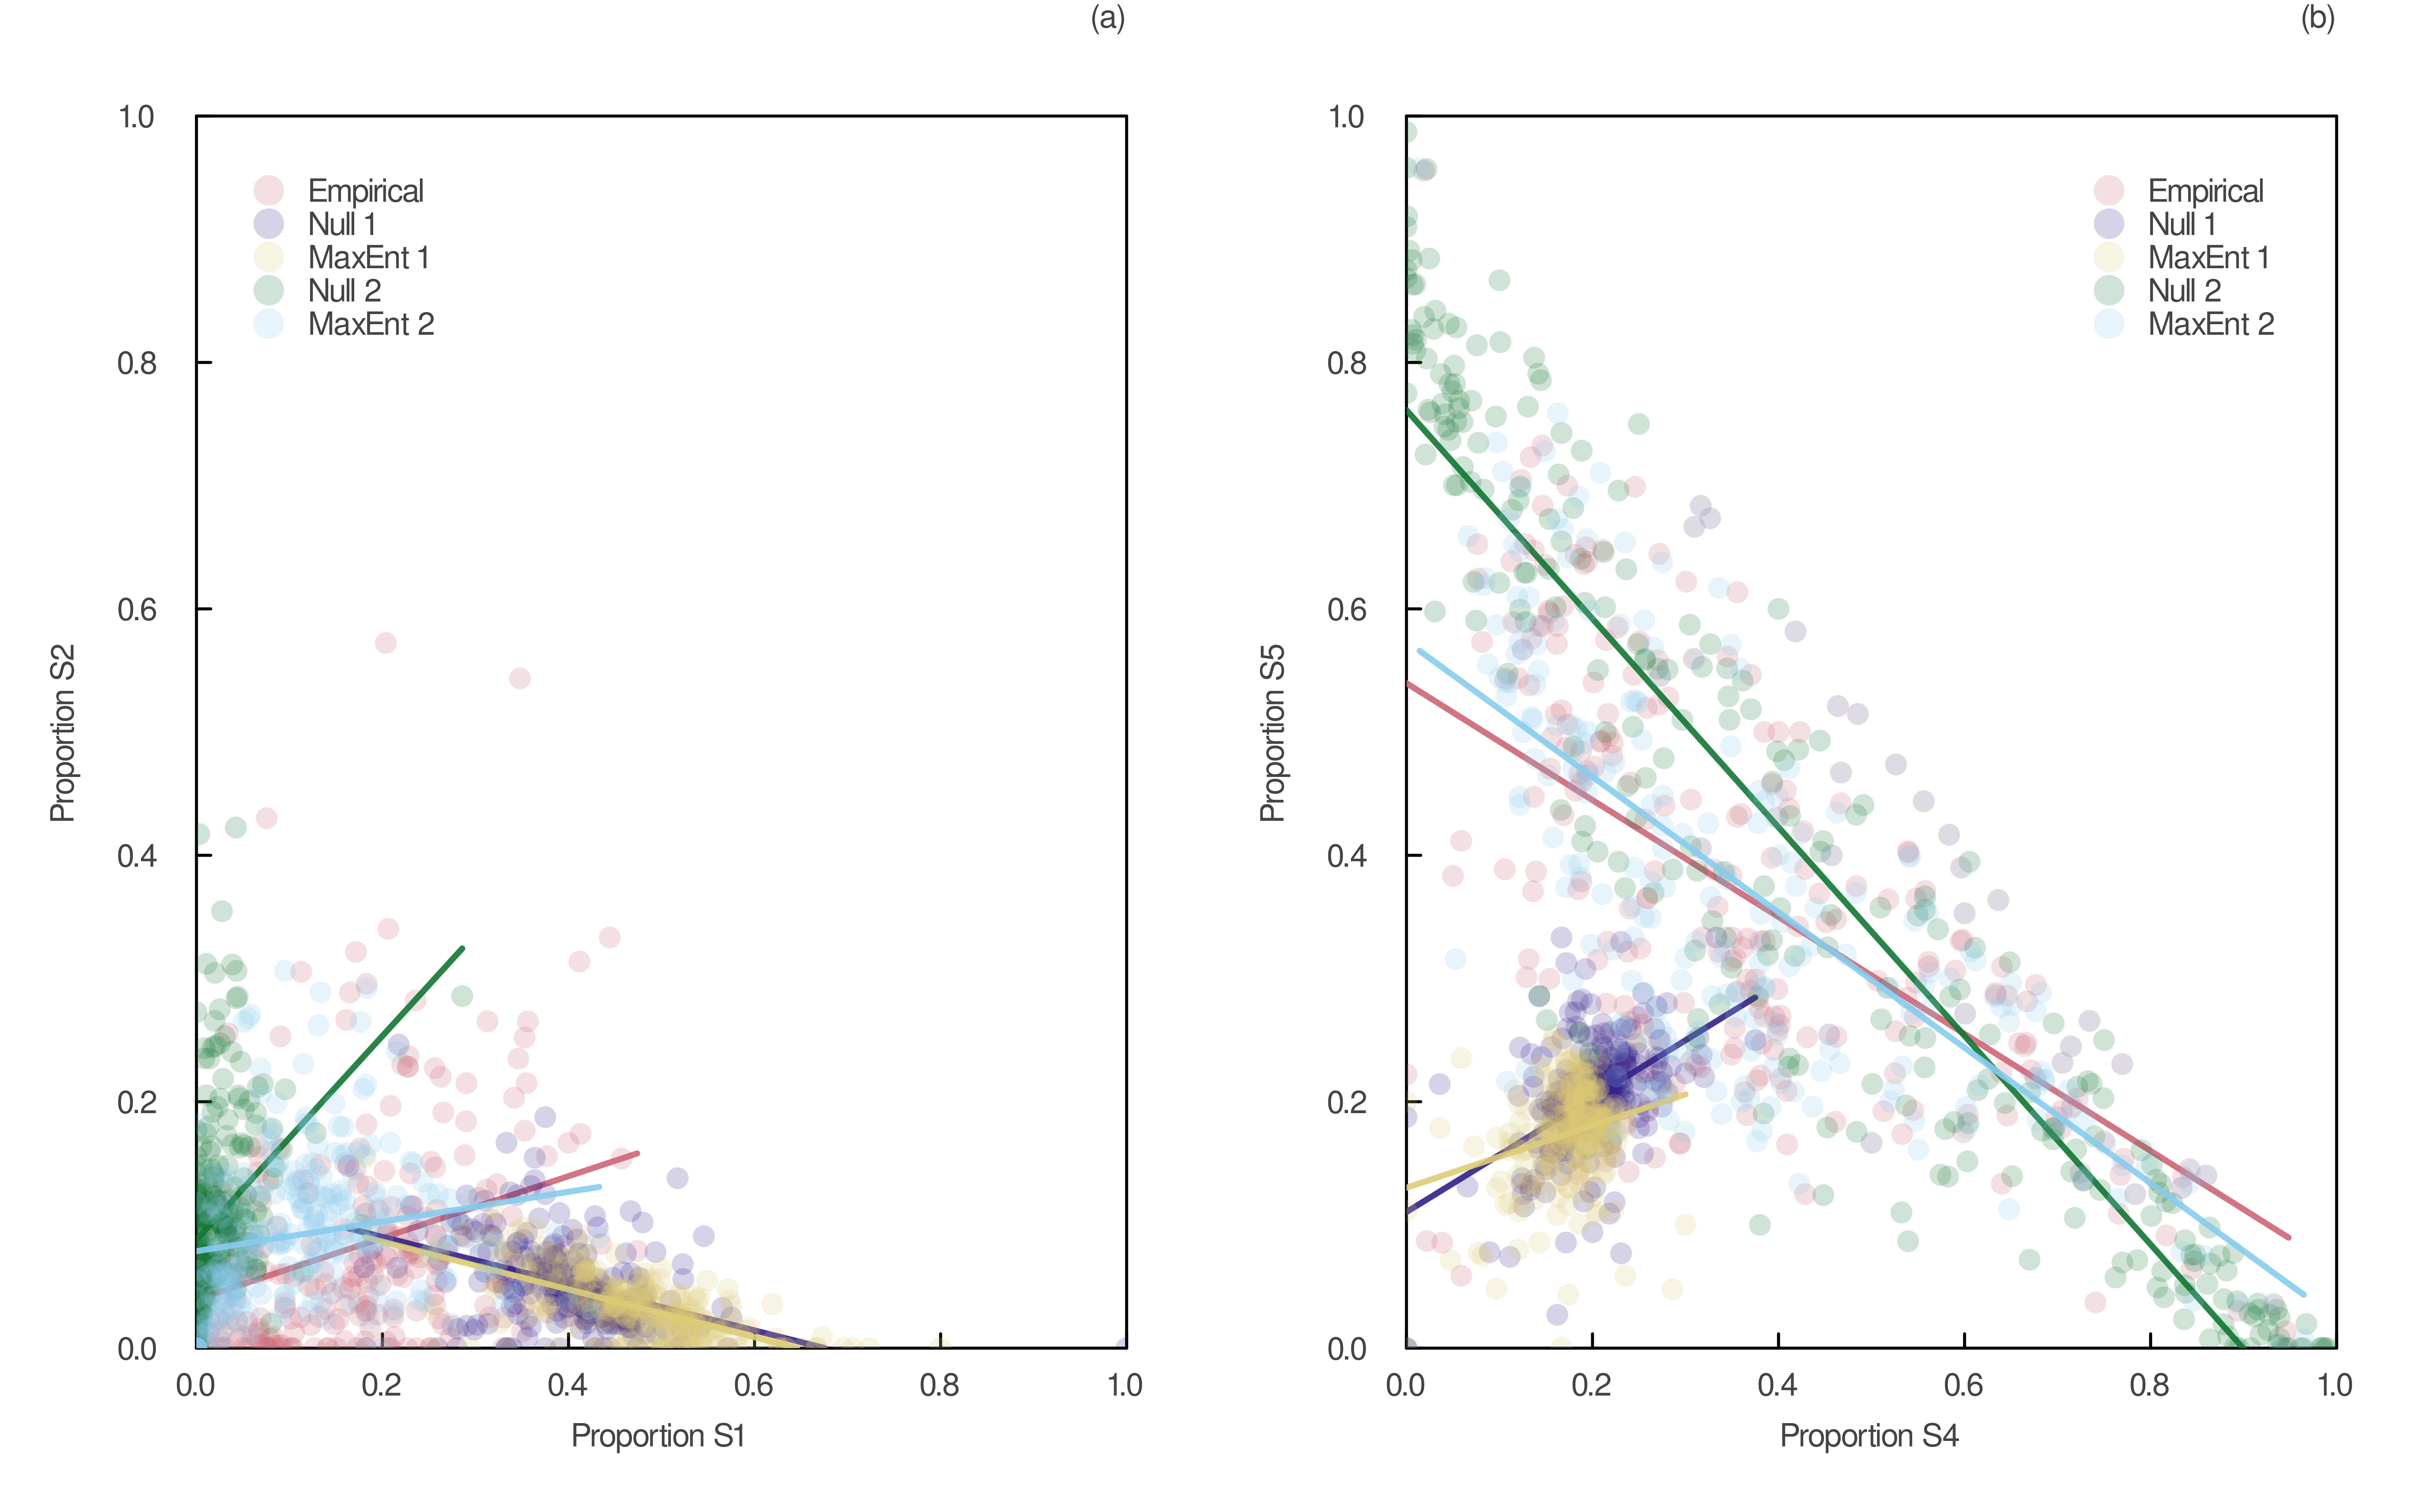
\includegraphics[width=\textwidth]{figures/article2/motifs_relations.png}
  \caption{\textbf{Pairwise relationships between the proportions of single-link three-species motifs in empirical and predicted food webs.}
    S1: Tri-trophic chain. S2: Omnivory. S4: Apparent competition. S5:
    Exploitative competition. Null 1: Type I null model based on connectance.
    MaxEnt 1: Type I heuristic MaxEnt model based on connectance. Null 2: Type
    II null model based on the joint degree sequence. MaxEnt 2: Type II
    heuristic MaxEnt model based on the joint degree sequence. Regression lines
    are plotted in each panel. Motif S3 is not shown because of its low
    proportion in most empirical and predicted networks.}
  \label{fig:motifs_rel}
\end{figure}

}

One of the challenges in implementing and validating a maximum entropy model is
to discover where its predictions break down. The results depicted in
Table~\ref{tbl:measures_all} and Figure~\ref{fig:measures} show that our type II heuristic
MaxEnt model can capture many high-level properties of food webs, but does a
poor job of capturing others. This suggests that, although the joint degree
sequence is an important driver of food-web structure, other ecological
constraints might be needed to account for some emerging food-web properties,
especially the ones regarding food-chain lengths. Nevertheless,
Figs~\ref{fig:motifs} and \ref{fig:motifs_rel} show that this model can reproduce
surprisingly well motif profiles, one of the most ecologically informative
properties of food webs. This suggests that the emerging structure of food webs
is mainly driven by their joint degree sequence, although higher-level
properties might need to be included in the model to ensure that food-chain
lengths fall within realistic values. 


\section{Conclusion}

The principle of maximum entropy is a mathematical method of finding
least-biased probability distributions that have some specified properties given
by prior knowledge about a system. We first applied this conventional MaxEnt
approach on food webs to predict species-level properties, namely the joint
degree distribution and the degree distribution of maximum entropy given known
numbers of species and interactions. We found that the joint degree
distributions of maximum entropy had a similar shape to the ones of empirical
food webs in high-connectance systems. However, these MaxEnt distributions were
more symmetric than the ones of empirical food webs when connectance was low,
which suggests that other constraints might be needed to improve these
predictions in low-connectance systems. Then, we used a slightly different
approach that aimed at finding heuristically the network configuration with the
highest SVD entropy, i.e. whose vector of relative singular values has maximum
entropy. This network of maximum entropy is the most complex, or random, given
the specified structure. We found that the heuristic maximum entropy model based
on connectance did not predict the structure of sampled food webs very well.
However, the heuristic maximum entropy model based on the entire joint degree
sequence, i.e. on the number of prey and predators for each species, gave more
convincing results. Indeed, this model reproduced food-web structure
surprisingly well, including the highly informative motif profile. Nevertheless,
it was not able to predict realistic food-chain lengths. 

Our results bring to the forefront the role of the joint degree distribution in
shaping food-web structure. This echoes the work of \textcite{Fortuna2010Nestedness},
who found that the degree distribution of ecological networks drives their
emerging structure such as their nestedness and modularity. Several measures of
food webs have been analyzed when studying the ecological consequences of
network structure (\cite{McCann2011Food}, \cite{Delmas2019Analysing}). In fact,
following \textcite{Williams2011Biology}, we believe that there is a lot more
ecological information in the deviation between these properties in empirical
systems and their maximum entropy configuration given a fixed joint degree
sequence.  

\subsection{Alternative MaxEnt models}

In this contribution, we used a method based on simulated annealing to find the
network configuration with the highest SVD entropy while fixing some aspects of
its structure. However, there are different ways to generate adjacency matrices
using MaxEnt. Another technique, also based on simulated annealing, could begin
by generating a food web randomly with fixed numbers of species and interactions
and calculating its joint degree distribution. Pairs of interactions could then
be swapped sequentially until we minimize the divergence between the calculated
joint degree distribution and the one of maximum entropy obtained analytically.
In that case, this is the entropy of the joint degree distribution that would be
maximized, not the one of the network's topology. To a certain extent, this
method would bridge the gap between the analytical and heuristic approaches
presented in this article. More research is needed to compare the quality of
different methods in generating adjacency matrices of food webs using MaxEnt.  

Maximum entropy graph models are another type of method that predicts a
distribution of adjacency matrices under soft or hard constraints (e.g.
\cite{Park2004Statistical}, \cite{Cimini2019Statistical}). Under hard
constraints, every network with a non-zero probability exactly satisfies the
constraints on its structure. This is in contrast with soft constraints, which
require that networks satisfy them on average (i.e. many networks with a
non-zero probability do not have the exact structure set by the constraints).
Maximum entropy graph models are helpful because they can provide probability
distributions for many network properties by measuring the structure of all
adjacency matrices with a non-zero probability. However, we consider that our
approach based on simulated annealing is more flexible and more computationally
efficient. Indeed, many measures of food-web structure are hard to translate
into mathematical constraints. Moreover, because food webs are directed networks
that can have self-loops, it makes the mathematical derivation of maximum
entropy graph models difficult. We believe that identifying heuristically what
constrains the topology of food webs is a useful first step before attempting to
derive the mathematical formulation of a maximum entropy graph model for food
webs. 

\subsection{Applications}

Our analytical and heuristic models can be applied for different purposes.
First, they could be used to generate first-order approximations of a network's
properties when state variables are known empirically. For example, knowing the
number of species in an ecological community, we can predict its number of
interactions using the flexible links model and then predict its joint degree
distribution with minimal biases using the principle of maximum entropy. This
could prove particularly useful when predicting network structure at large
spatial scales, subdividing the study area into smaller communities (e.g. grid
cells). Indeed, because species richness and other ecological data are
increasingly abundant (e.g. \cite{Dickinson2010Citizen}), validated MaxEnt models
can be used to respond to a wider range of macroecological questions regarding
food webs. 

Second, our analytical model can be used to generate informative priors in
Bayesian analyses of the structure of ecological networks (e.g.
\cite{Cirtwill2019Quantitative}). Indeed, the probability distribution of maximum
entropy derived using MaxEnt can be used as a prior that can be updated with
novel data. For instance, if we know the number of species and the number of
interactions, we can derive the degree distribution of maximum entropy, as shown
in this contribution. The degree distribution represents the probability that a
species can interact (as a predator or a prey) with a given number of other
species. Data on species interactions can be used to update the prior degree
distribution to generate a more accurate posterior distribution, thus improving
our description and understanding of the system.

Third, our analytical and heuristic models can be used to make better
predictions of pairwise species interactions by constraining the space of
feasible networks, as discussed in \textcite{Strydom2021Roadmapa}. In other words, we
can use the network configuration or specific measures of food-web structure
derived using MaxEnt to ensure that our predictions of interspecific
interactions form feasible networks. This means that the probability that two
species interact may be conditional on the network structure and the probability
of interactions of all other species pairs. When data are limited, MaxEnt can be
used to predict network structure on which pairwise probabilities of
interactions are conditional.

Finally, our analytical and heuristic models can be used as alternative null
models of ecological networks to better understand and identify the ecological
processes driving food-web structure. Indeed, these mechanisms can be better
described when analyzing the deviation of empirical data from MaxEnt predictions
(\cite{Caruso2022Fluctuating}). A strong deviation would indicate that ecological
mechanisms not captured by the statistical constraints are at play for the
system at hand. For instance, the incapacity of a MaxEnt model to reliably
predict entropy may be a compelling indication of additional constraints shaping
food-web structure. If deviations are systematic, the maximum entropy model
might need to be revised to include appropriate ecological constraints. This
revision process helps us reflect on and identify what constrains food-web
structure. However, it is important to note that tangible ecological mechanisms
cannot be directly inferred from statistical distributions
(\cite{WarrenII2022Seeing}). Instead, by identifying the constraints of a
system and by analyzing empirical deviations from maximum entropy predictions,
MaxEnt can only help us redirect research efforts toward understanding the
biological mechanisms behind these constraints. 

The principle of maximum entropy can thus be applied to both the prediction and
understanding of natural systems. The model's interpretation depends on how we
use it. It can be used as a baseline distribution to identify the ecological
processes organizing natural systems. It can also be used to generate
predictions of ecological networks. This distinction between understanding and
predicting is important when using and interpreting MaxEnt models. 

\subsection{Final remarks}

One of the biggest challenges in using the principle of maximum entropy is to
identify the set of state variables that best reproduce empirical data. We found
that the number of species and the number of interactions are important state
variables for the prediction of the joint degree distribution. Similarly, we
found that the numbers of prey and predators for each species in a food web are
important state variables for the prediction of the network configuration.
However, our predictions overestimated the symmetry of the joint degree
distribution for our analytical model and the maximum trophic level and network
diameter for our heuristic model. We should thus continue to play the ecological
detective to find these other topological constraints that would improve the
predictions of MaxEnt models and help us understand better what drives food-web
structure.

\section{Acknowledgments}

We acknowledge that this study was conducted on land within the traditional
unceded territory of the Saint Lawrence Iroquoian, Anishinabewaki, Mohawk,
Huron-Wendat, and Omàmiwininiwak nations. This work was supported by the
Institute for Data Valorization (IVADO, PhD-2019a-5993304626), which supported
FB, and the Natural Sciences and Engineering Research Council of Canada (NSERC)
Collaborative Research and Training Experience (CREATE) program, through the
Computational Biodiversity Science and Services (BIOS2) program, which supported
FB, DG, and TP. TP received funding from the Canadian Institute for Ecology and
Evolution and a donation from the Courtois Foundation. TP also acknowledges
financial support from NSERC through the Discovery Grants and Discovery
Accelerator Supplement programs. 

 % Pour générer la bibliographie à la fin
 % de l'article, utiliser la commande de la
 % classe <dms> \sectionbibliography{<nom du .bib>}.
 % Il y a aussi la possibilité d'utiliser le package
 % <chapterbib>, auquel cas on utilise simplement
 % \bibliography normalement.
 %
 % IMPORTANT : Dans tous les cas, il faut faire
 %    pdflatex these
 %    bibtex chapitre1
 %    bibtex chapitre2
 %    .
 %    .
 %    .
 %    bibtex chapitreN
 %    pdflatex these
 %    pdflatex these
 %
 % où <these> est le nom du .tex principal
 % (qui contient le \documentclass).
 % bibtex a besoin du .aux de chapitre1 et
 % non du .tex. Il est parfois nécessaire
 % d'effacer le .aux et de recommencer la
 % compilation du début.
%%\bibliographystyle{amsplain} % style plain anglais ou
%% \bibliographystyle{amsplain-french} % style plain francais
%%\bibliographystyle{<style>} % autre
%% \sectionbibliography{ref.bib} %Donner le nom du .bib

\endinput
%%
%% End of file `03_article2.tex'.
